%Dies ist die Hauptseite des Dokumentes. Es werden u. a. alle Kapitel,
%Einstellung im Header eingebunden.  Veränderungen müssen in folgenden Dateien
%vorgenommen werden:
      %- config.tex
      %- einzelne Kapitel (evtl. erweitern)

%Hier sind alle Einstellungen enthalten, die sich auf das Seiten- und
%Dokumentenlayout beziehen

\documentclass[
  11pt,                   % Schriftgröße
  DIV12,
  german,                 % für Umlaute, Silbentrennung etc.
  oneside,                % einseitiges Dokument
  titlepage,              % es wird eine Titelseite verwendet
  parskip=half,           % Abstand zwischen Absätzen (halbe Zeile)
  headings=normal,        % Größe der Überschriften verkleinern
  captions=tableheading,  % Beschriftung von Tabellen unterhalb ausgeben
  final                   % Status des Dokuments (final/draft)
]{scrreprt}               %


%------Ändern von Schriftschnitten - (Muss ganz am Anfang stehen !) ------------
\usepackage{fix-cm}


%------Umlaute -----------------------------------------------------------------
%   Umlaute/Sonderzeichen wie äüöß können direkt im Quelltext verwenden werden.
%    Erlaubt automatische Trennung von Worten mit Umlauten.
\usepackage[T1]{fontenc}
\usepackage[utf8]{inputenc}

%------Anpassung der Landessprache----------------------------------------------
\usepackage[ngerman]{babel}

%------Einfache Definition der Zeilenabstände und Seitenränder------------------
\usepackage{geometry}
\usepackage{setspace}

%------Schriftgrößenanpassung von einzelnen Textpassagen------------------------
\usepackage{relsize}

%------Trennlinien in Kopf- und Fusszeile
\usepackage[headsepline, footsepline, ilines]{scrlayer-scrpage}

%------Grafiken und Farben -----------------------------------------------------
\usepackage{graphicx}

%------Packet zum Sperren, Unterstreichen und Hervorheben von Texten------------
\usepackage{soul}

%------ergänzende Schriftart----------------------------------------------------
\usepackage{helvet}

%------Lange Tabellen-----------------------------------------------------------
\usepackage{longtable}
\usepackage{array}
\usepackage{ragged2e}
\usepackage{lscape}
\usepackage{tabularx}

%------DocTeX-------------------------------------------------------------------
\usepackage{changepage}
\usepackage{scalerel}
\newcolumntype{R}{>{\raggedright\arraybackslash}X}%

%------PDF-Optionen-------------------------------------------------------------
\usepackage[
  bookmarks,
  bookmarksopen=true,
  colorlinks=true,
  linkcolor=black,        % einfache interne Verknüpfungen
  anchorcolor=black,      % Ankertext
  citecolor=black,        % Verweise auf Literaturverzeichniseinträge im Text
  filecolor=black,        % Verknüpfungen, die lokale Dateien öffnen
  menucolor=black,        % Acrobat-Menüpunkte
  urlcolor=black,         % Farbe für URL-Links
  backref,                % Zurücktext nach jedem Bibliografie-Eintrag als
                          % Liste von Überschriftsnummern
  pagebackref,            % Zurücktext nach jedem Bibliografie-Eintrag als
                          % Liste von Seitenzahlen
  plainpages=false,       % zur korrekten Erstellung der Bookmarks
  pdfpagelabels,          % zur korrekten Erstellung der Bookmarks
  hypertexnames=false,
  colorlinks=true,   % zur korrekten Erstellung der Bookmarks
  linktocpage             % Seitenzahlen anstatt Text im Inhaltsverzeichnis verlinken
  ]{hyperref}
  \hypersetup{
    colorlinks=true, %set true if you want colored links
    linktoc=all,     %set to all if you want both sections and subsections linked
  }
  \usepackage{verbatim}
  \usepackage{lipsum}                     % Dummytext
  \usepackage{xargs}                      % Use more than one optional parameter in a new commands
  \usepackage[pdftex,dvipsnames]{xcolor}  % Coloured text etc.

  \usepackage[colorinlistoftodos,prependcaption,textsize=tiny]{todonotes}

%------Glossar------------------------------------------------------------------
\usepackage[translate=babel,toc]{glossaries}
      % enthält eingebundene Packete

%------Seitenränder-------------------------------------------------------------
\geometry{verbose,                     % zeigt die eingestellten Parameter beim
                                       % Latexlauf an
      paper=a4paper,                   % Papierformat
      top=25mm,                        % Rand oben
      left=25mm,                       % Rand links
      right=25mm,                      % Rand rechts
      bottom=45mm,                     % Rand unten
      pdftex                           % schreibt das Papierformat in die
                                       % Ausgabe damit Ausgabeprogramm
                                       % Papiergröße erkennt
  }

%Seitenlayout
\onehalfspace        % 1,5-facher Abstand

%------Kopf- und Fußzeilen -----------------------------------------------------
\pagestyle{scrheadings}

%------Kopf- und Fußzeile auch auf Kapitelanfangsseiten ------------------------
\renewcommand*{\chapterpagestyle}{scrheadings}

%------Schriftform der Kopfzeile -----------------------------------------------
\renewcommand{\headfont}{\normalfont}

%----Spezielle Befehle
\newcommand{\lfk}[1]{$\langle LF#1\rangle$}

%----Farben
\definecolor{tubsRed}{cmyk}{0.1,1.0,0.8,0.0}
\definecolor{tuRed}{cmyk}{1.0,0.0,0.6,0.0}

%------Kopfzeile----------------------------------------------------------------
\setheadsepline{1pt}[\color{tuRed}]
\setlength{\headheight}{21mm}        % Höhe der Kopfzeile
\ihead{\large{\textsc{\praktikumTitel}}\\    % Text in der linken Box
       \small{\projektTitel}}
\chead{}                            % Text in der mittleren Box

%----Fusszeile
\setfootsepline{1pt}[\color{tuRed}]
\cfoot{}                            % Text in mittlerer Box
\ofoot{\pagemark}                    % Seitenzahl in rechter Box



%------Labels mit eigenem Text für \ref ----------------------------------------
\makeatletter
\def\namedlabel#1#2{\begingroup
#2%
\def\@currentlabel{#2}%
\phantomsection\label{#1}\endgroup
}
\makeatother


%------Neue Environments -------------------------------------------------------

\newcommand{\refsetcounter}[2]{\setcounter{#1}{#2}\addtocounter{#1}{-1}\refstepcounter{#1}}

%%Funktion im Pflichtenheft
%\newcounter{functioncount}
%\newenvironment{function}[2]{\refsetcounter{functioncount}{#1}\large\textbf{\sffamily{#2 }}\namedlabel{F#1}{$\langle F#1\rangle$}\normalsize\begin{description}\setlength{\itemsep}{-5pt}}{\end{description}}
%
%%Daten im Pflichtenheft
%\newcounter{datacount}
%\newenvironment{data}[2]{\refsetcounter{datacount}{#1}\textbf{#2} \namedlabel{D#1}{$\langle D#1\rangle$}\\}{}
%
%Kriterien im Pflichtenheft
\newcounter{mustcount}
\newcommand{\must}[2]{\refsetcounter{mustcount}{#1}\namedlabel{MK#1}{$\langle MK#1\rangle$}~#2\\}

\newcommand{\mustchange}[2]{\ref{MK#1}~#2 \\}

\newcounter{wishcount}
\newcommand{\wish}[2]{\refsetcounter{wishcount}{#1}\namedlabel{WK#1}{$\langle WK#1\rangle$}~#2\\}

\newcommand{\wishchange}[2]{\ref{WK#1}~#2 \\}


%
%\newcounter{wontcount}
%\newcommand{\wont}[2]{\refsetcounter{wontcount}{#1}\namedlabel{RN#1}{$\langle AK#1\rangle$} #2\\}
%
%\newcounter{notfunctional}
%\newcommand{\notfunctional}[2]{\refsetcounter{notfunctional}{#1}\namedlabel{NF#1}{$\langle NF#1\rangle$} #2\\}
%
%%Qualitätsanforderungen im Pflichtenheft
%\newcommand{\qualityReq}[2]{\refsetcounter{datacount}{#1}\namedlabel{Q#1}{$\langle Q#1\rangle$} #2\\}

% Benutzeroberflächen im Pflichtenheft
\newcounter{uicount}
\newenvironment{ui}[2]{\refsetcounter{uicount}{#1}\textbf{#2} \namedlabel{UI#1}{$\langle UI#1\rangle$}\\}{}

% Klassen
\newcounter{classcount}
\newenvironment{class}[2]{\refsetcounter{classcount}{#1}\textbf{#2}\namedlabel{CL#1}{$\langle CL#1\rangle$}\begin{description}\setlength{\itemsep}{-5pt}}{\end{description}}

% Entitäten
\newcounter{entitycount}
\newenvironment{entity}[2]{\refsetcounter{entitycount}{#1}\textbf{#2} \namedlabel{E#1}{$\langle E#1\rangle$}\\}{}

% Component
\newcounter{componentcount}
\newenvironment{component}[2]{\refsetcounter{componentcount}{#1}\textbf{Komponente \namedlabel{C#1}{$\langle C#1\rangle$}: #2}\\}{}

% Interface
\newcounter{interfacecount}
\newenvironment{interface}[2]{\refsetcounter{interfacecount}{#1}\textbf{Schnittstelle \namedlabel{I#1}{$\langle I#1\rangle$}: #2}\\}{}

% Testfall
\newcounter{scenariocount}
\newenvironment{scenario}[2]{\refsetcounter{scenariocount}{#1}\textbf{Szenario: #2}\namedlabel{S#1}{$\langle S#1\rangle$}\normalsize\begin{description}\setlength{\itemsep}{-5pt}}{\end{description}\hspace{7.5em}}
           % Diese Datei enthält alle
                                           % Layouteinstellungen
\newcommand{\dokumentTitel}{Pflichtenheft}
% Definition von globalen Parametern, die derzeit auf der Titelseite und in der
% Kopfzeile verwendet werden. Der in <> gesetzte Text ist zu verändern.

\newcommand{\praktikumTitel}{Praxis der Softwareentwicklung}
\newcommand{\projektTitel}{Solidarische Raumnutzung}

\newcommand{\semester}{Wintersemester 2024/25}
\newcommand{\institut}{
	Institut für Anthropomatik und Robotik (IAR)\\
	Forschungsgruppe Mensch-Maschine-Interaktion und Barrierefreiheit (MBI)\\
	Prof. Dr. Kathrin Gerling\\
	Adenauerring 10, Gebäude 50.28\\
	76131 Karlsruhe\\
}
\newcommand{\institutsLogo}{common/hci.jpg}
\newcommand{\kitlogo}{common/kit_logo.jpg}
\newcommand{\betreuer}{Sabrina Burtscher, Dmitry Alexandrovsky}


\newcommandx{\unsure}[2][1=]{\todo[linecolor=red,backgroundcolor=red!25,bordercolor=red,#1]{#2}}
\newcommandx{\change}[2][1=]{\todo[linecolor=blue,backgroundcolor=blue!25,bordercolor=blue,#1]{#2}}
\newcommandx{\info}[2][1=]{\todo[linecolor=OliveGreen,backgroundcolor=OliveGreen!25,bordercolor=OliveGreen,#1]{#2}}
\newcommandx{\improvement}[2][1=]{\todo[linecolor=Plum,backgroundcolor=Plum!25,bordercolor=Plum,#1]{#2}}
\newcommandx{\thiswillnotshow}[2][1=]{\todo[disable,#1]{#2}}

\makeglossaries

%------Beginn des Gesamtdokumentes----------------------------------------------
\begin{document}

%------Eingebundene Seiten, Verzeichnisse bzw. Kapitel--------------------------
% Dies ist die Titelseite.
% Die Ausgabe darf 1 Seite nicht überschreiten, also ggf. Abstände anpassen
% Die Angabe in [...] gibt den Abstand nach der entsprechenden Zeile an.


%----Stil dieser Seite----------------------------------------------------------
\thispagestyle{plain}      % Kopfzeile bleibt leer

%----Beginn der Titelseite------------------------------------------------------
\begin{titlepage}

\vspace*{-3.8cm}
\hspace*{-2cm}\begin{minipage}{1.25\textwidth}

\includegraphics[width=5.3cm]{common/kit_logo}\setlength{\unitlength}{1mm}\begin{picture}(00,00)(-10,0)\color{tuRed}\put(000,004){\line(1,0){140}}\end{picture}%\hfill
\parbox[b]{0.68\textwidth}{\hfill\includegraphics[width=8cm,height=2.4cm,keepaspectratio]{\institutsLogo}\\~}
\end{minipage}


~\\[5ex]

%----zentrierte Ausrichtung über die gesamte Seite----------------------------
\begin{center}

%----Titel des Praktikum (\praktikumTitel in newComments zu verändern)--------
{\relsize{4}{\textbf{\textsc{\praktikumTitel}}}}\\[5ex]

%----Titel des Teilprojektes (\projektTitel in newComments verändern)---------
{\relsize{3}{\textbf{\textsc{\projektTitel}}}}\\[5ex]

Praxis der Softwareentwicklung (PSE)\\
\semester\\[6ex]

{\relsize{3}{\textbf{\dokumentTitel}}}\\[5ex]

%----Daten des Auftraggebers
Karlsruher Institut für Technologie (KIT)\\
\institut[2ex]
\textbf{Betreuer: \betreuer}\\[5ex]

\textbf{Projektteilnehmer:}\\

% ----Tabelle der Praktikumsteilnehmer------------------------------------------
\begin{tabular}{l<{\hspace{20mm}} l<{\hspace{30mm}}}\\
  Name                   &   E-Mail-Adresse\\      % Zeilenüberschift

  \hline                    % Linie unterhalb der Zeilenüberschrift

  %----Nachfolgend alle Namen und E-Mail-Adressen der Teilnehmer einfügen
  Antonia Ammon  &  uipkm@student.kit.edu\\
  Ben Steinle &  ufikl@student.kit.edu\\
  Johannes Frohnmeyer &  uczkf@student.kit.edu\\
  Alexander Klee &  ukvpq@student.kit.edu\\
  Jannik Hönlinger &  uouyo@student.kit.edu\\

\end{tabular}

%Zur Vereinheitlichung sollten hier die TU Braunschweig Emailadressen benutzt werden. % enthält Tabelle der Praktikumsteilnehmer

\vfill
Karlsruhe, \today

\end{center}
\end{titlepage}
                       % Titelseite

\newglossaryentry{CI}{name=CI/CD, description={Baut automatisiert Software, führt Tests durch und veröffentlicht Artefakte}}
\newglossaryentry{Docker}{name=Docker, description={Software zur Bereitstellung von Anwendungen innerhalb von Containern}}
\newglossaryentry{Container}{name=Container, description={Isolierte Umgebung um Software unabhängig von der zugrunde liegenden Umgebung auszuführen}}
\newglossaryentry{Devcontainer}{name=Devcontainer, description={Container, welcher eine Entwicklungsumgebung bereitstellt}}
\newglossaryentry{Browser}{name=Browser, description={Software zum Navigieren von Webseiten, zum Beispiel Firefox oder Chrome}}
\newglossaryentry{Git}{name=Git, description={Software zur Versionsverwaltung von Softwareprojekten}}
\newglossaryentry{GitHub}{name=GitHub, description={Plattform zur Versionsverwaltung von Softwareprojekten, nutzt Git}}
\newglossaryentry{IDE}{name=IDE, description={(Integrated Development Environment) Software, welche alle Werkzeuge zur Softwareentwicklung in einem Programm kombiniert}}
\newglossaryentry{AMD64}{name=AMD64, description={Verbreitete Prozessorarchitektur von Intel und AMD}}
\newglossaryentry{RAM}{name=RAM, description={\ (Random Access Memory) Arbeitsspeicher}}
\newglossaryentry{VM}{name=VM, description={\ (Virtuelle Maschine) Software zur Simulation eines Computers}}
\newglossaryentry{PostgreSQL}{name=PostgreSQL, description={Objekt-Relationales Datenbankmanagementsystem, welches zum Speichern und Verwalten von Daten verwendet wird}}
\newglossaryentry{HTML}{name=HTML, description={\ (Hypertext Markup Language) Eine Sprache, um die Struktur und den Inhalt einer Website zu definieren}}
\newglossaryentry{CSS}{name=CSS, description={Cascading Style Sheets, ist eine Sprache um das Visuelle aussehen einer Website zu definieren}}
\newglossaryentry{JavaScript}{name=JavaScript, description={Programmiersprache um das Logische verhalten von Webseiten zu steuern}}
\newglossaryentry{SSR}{name=SSR, description={(Server-Side Rendering) Methode, um das HTML einer Website auf dem Server zu produzieren, statt im Browser}}
\newglossaryentry{REST}{name=REST, description={\ (Representational State Transfer) Architekturstil von APIs für das Internet}}
\newglossaryentry{API}{name=API, description={Schnittstelle auf Quelltext-Ebene um anderen Programmen funktionen zur Verfügung zu stellen}}
\newglossaryentry{UI}{name=UI, description={(User Interface) Typischerweise visuelle Oberfläche, mit welcher der Nutzende interagiert}}
\newglossaryentry{OIDC}{name=OIDC, description={\ (OpenID Connect) Authorisierungsframework welches vom KIT genutzt wird um dritten Webseiten Logins basierend auf KIT-Konten bereitzustellen}}
\newglossaryentry{Gradle}{name=Gradle, description={Build-Management-Tool welches auf Java basiert}}
\newglossaryentry{iCal}{name=iCal, description={Dateiformat zur Speicherung von Kalenderdaten}}
\newglossaryentry{WCAG}{name=WCAG, description={\ (Web Content Accessibility Guidelines) Standard zur Barrierefreien gestaltung von Webseiten.}}

\tableofcontents                           % Inhaltsverzeichnis wird automatisch
                                           % generiert
\listoffigures
\newpage
%\listoftodos[Notes]
%----Kapitel des Pflichtenhefts, die mit Inhalt zu füllen sind--------------------
%!TEX root = ../Pflichtenheft.tex
\chapter{Einleitung}
In modernen und inklusiven Arbeits- und Lernumgebungen spielen Rückzugsorte eine zentrale Rolle um produktives Arbeiten und das Wohlbefinden aller gewährleisten zu können.
Das Institut für Mensch-Maschine-Interaktion und Barrierefreiheit (MIB) am KIT bietet einen Ruheraum, welcher für Meetings, kurzen Pausen oder als Rückzugsort nach einer Reizüberflutung genutzt werden kann.

Derzeit wird der Status des Raumes durch ein einfaches Türschild angezeigt, welches lediglich den Status \textit{verfügbar} oder \textit{besetzt} anzeigt.
Dieses System bietet jedoch keine Möglichkeit, die Dringlichkeit sowie die Nutzung zu kommunizieren und zu planen.

Im Rahmen dieses Projekts wird ein innovatives Buchungssystem entwickelt, das über ein klassisches \textit{frei}- oder \textit{gebucht}-System hinausgeht.
Ziel ist es, ein System zu schaffen, das es den Nutzenden ermöglicht, ihre Bedürfnisse differenziert anzugeben.
Dadurch soll eine transparente und flexible Abstimmung über die Raumnutzung ermöglicht werden, die sowohl individuellen Bedürfnissen als auch einer optimalen Raumverteilung gerecht wird.
%!TEX root = ../Pflichtenheft.tex

\chapter{Zielbestimmung}
\label{chap:target}


\section{Musskriterien}\label{sec:musskriterien}

\must{1}{Die Anwendung muss als Web-Applikation realisiert werden.}
\must{2}{Nutzende der Anwendung müssen sich mit ihrem KIT-Konto per \gls{OIDC} oder einem lokalen Gastkonto anmelden können.}
\must{3}{Nutzende müssen sich abmelden können.}
\must{4}{Die Anwendung muss die Ansichten Kalender, Termin, Termin-erstellen, Login, Kontenliste und Terminübersicht anbieten.}
\must{5}{Die Ansicht \textit{Kalender} muss einen klaren Überblick über die bereits reservierten Zeiten geben.}
\must{6}{Die Ansicht \textit{Kalender} muss die Öffnungszeiten des Raumes darstellen.}
\must{7}{Die Ansicht \textit{Kalender} muss die Termine des/r angemeldeten Nutzenden hervorgehoben darstellen.}
\must{8}{Die Ansicht \textit{Termin} muss die Möglichkeit bieten, genauere Informationen über einen Termin darzustellen.}
\must{9}{Die Ansicht \textit{Termin-Erstellen} muss die Möglichkeit bieten, einen Raum für eine bestimmte Zeitperiode zu reservieren.}
\must{10}{Bei der Reservierung eines Raumes muss optional die Möglichkeit bestehen eine Beschreibung zu hinterlegen. Hierbei müssen die Nutzenden klar darauf hingewiesen werden, wer diese Daten einsehen kann.}
\must{11}{Die Terminübersicht muss den Nutzenden die Möglichkeit bieten, all ihre Termine zu verwalten.}
\must{12}{Die Priorität eines Termins ist in drei Stufen gegliedert.}
\must{13}{Beim Erstellen eines Termins wählen die Nutzenden aus, ob sie ihren Raum mit anderen Personen teilen möchten. Dabei stehen die Optionen \textit{Ja}, \textit{Nein} und \textit{Auf Anfrage} zur Auswahl.}
\must{14}{Die Anwendung muss Terminkonflikte reibungslos mithilfe der Prioritäten lösen können. Dabei überschreiben Termine mit höherer Priorität andere.}
\must{15}{Die Anwendung muss in der Lage sein, Nutzende per E-Mail darüber zu informieren, wenn ihr Termin durch einen Termin mit höherer Priorität überschrieben wurde.}
\must{16}{Nutzende der Anwendung müssen in der Lage sein, eine Reservierung zu stornieren.}
\must{17}{Es muss ein Adminkonto geben, welches per Passwort authentifiziert wird. Nur der Server-Admin darf dieses Passwort ändern können.}
\must{18}{Die Ansicht \textit{Kontoliste} muss den Admins die Möglichkeit bieten, einzelne Konten sowie die Anmeldung per Gastkonto zu deaktivieren.}
\must{19}{Admins müssen in der Ansicht \textit{Termin} Termine löschen können.}
\must{20}{Es muss ein farbcodiertes Banner geben, der den aktuellen Status des Raumes anzeigt.}
\must{21}{Admins müssen in der Ansicht \textit{Kalender} die Öffnungszeiten einstellen können}


\section{Wunschkriterien}\label{sec:wunschkriterien}

\wish{1}{Es könnte die Möglichkeit geben, mehr als einen Raum zur Buchung anzubieten. Dabei könnte eine Raumauswahl vor der Ansicht \textit{Kalender} die verschiedenen Möglichkeiten präsentieren. Existiert nur ein Raum, wird diese Auswahl übersprungen.}
\wish{2}{In der Ansicht \textit{Kalender} könnten Feiertage automatisch eingebunden werden.}
\wish{3}{Admins könnten die Möglichkeit haben, geplante Wartungs- und Sperrzeiten einzurichten.}
\wish{4}{Termine könnten nach der Buchung im \gls{iCal}-Format zum Export angeboten werden.}
\wish{5}{Nutzende könnten in der Ansicht \textit{Termin} die Möglichkeit haben, ihre eigenen Termine zu bearbeiten.}
\wish{6}{Die Ansicht \textit{Kalender} könnte visualisieren, welche Termine bereits in der Vergangenheit liegen und wo der Übergang von der Vergangenheit zur Zukunft liegt.}
\wish{7}{Tooltips könnten Nutzenden erklären, wofür bestimmte Elemente der \gls{UI} verwendet werden.}
\wish{9}{Es könnte einen physischen Panik-Button geben.}
\wish{10}{Die Anwendung könnte in der Lage sein, Nutzende zu informieren, falls ein gewünschter Termin frei wird.}
\wish{11}{Es könnte einen Quick-Checkin-Button geben, welcher eine vorausgefüllte Terminerstellung öffnet. Dieser bietet auch eine Alternative zur Interaktion mit dem Kalender.}
\wish{12}{Es könnte einen Quick-Checkout-Button geben, der vorzeitiges Beenden eines Termines ermöglicht.}
\wish{13}{Admins könnten eine Statistik-Ansicht nutzen.}


\section{Abgrenzungskriterien}\label{sec:abgrenzungskriterien}

\wont{1}{Die Verteilung von Buchungen zwischen ähnlichen Räumen ist nicht Teil des Projekts.}
\wont{2}{Das Skalieren der Anwendung auf eine große Anzahl von Räumen ist nicht vorgesehen.}
\wont{3}{Die Buchung von Räumen für mehrere Tage ist nicht vorgesehen.}
\wont{4}{Die Verwaltung von Räumen, die mehrere Arbeitsplätze umfassen, ist nicht vorgesehen.}
\wont{5}{Die Entwicklung plattformspezifischer Anwendungen und der dafür notwendigen \gls{API}s ist nicht vorgesehen.}
\wont{6}{Die Reservierung ist nur für die nahe Zukunft gedacht, eine Langzeitplanung ist nicht vorgesehen.}
\wont{7}{Die Reservierung wiederholter Termine ist nicht vorgesehen.}
\wont{8}{E-Mail-Adressen von Gastkonten werden nicht verifiziert.}
%!TEX root = ../Pflichtenheft.tex

\chapter{Produktübersicht}
\label{chap:product_overview}
Um sich einen Überblick über die im Produkt enthaltenen Funktionen zu verschaffen, wird in diesem Kapitel eine Übersicht über die grundlegenden Funktionen in Form von Aktivitätsdiagrammen gegeben.
Zudem werden die Betriebsbedingungen beschrieben.
\section{Betriebsbedingungen}
\begin{itemize}
    \item Die Software soll in einem \gls{Docker}-\gls{Container} laufen.
    \item Die Software soll weitgehend ohne Unterbrechung laufen.
    \item Ständige Wartung ist nicht vorgesehen, die Software soll weitgehend autonom laufen.
    \item Übliche Administrationsaufgaben sollen über die Administrationsoberfläche und ohne Neustart der Software möglich sein.
    \item Die \gls{RAM}-Nutzung soll möglichst gering sein (Ideal: unter 1GB)
\end{itemize}

\newpage
\section{Aktivitätsdiagramm-Diagramme}

\subsection{Admin Funktionalität}
In Abbildung \ref{fig:activity_diagram_admin} ist das Aktivitätsdiagramm für die Admin-Funktionalität dargestellt,
welches die Musskriterien \ref{MK3}, \ref{MK4}, \ref{MK17}, \ref{MK18} und \ref{MK19} abdeckt,
sowie die Produktfunktionen \ref{F100}, \ref{F10}, \ref{F30}, \ref{F50}, \ref{F60}, \ref{F90} und \ref{F110}.
\begin{figure}[ht]
    \centering
    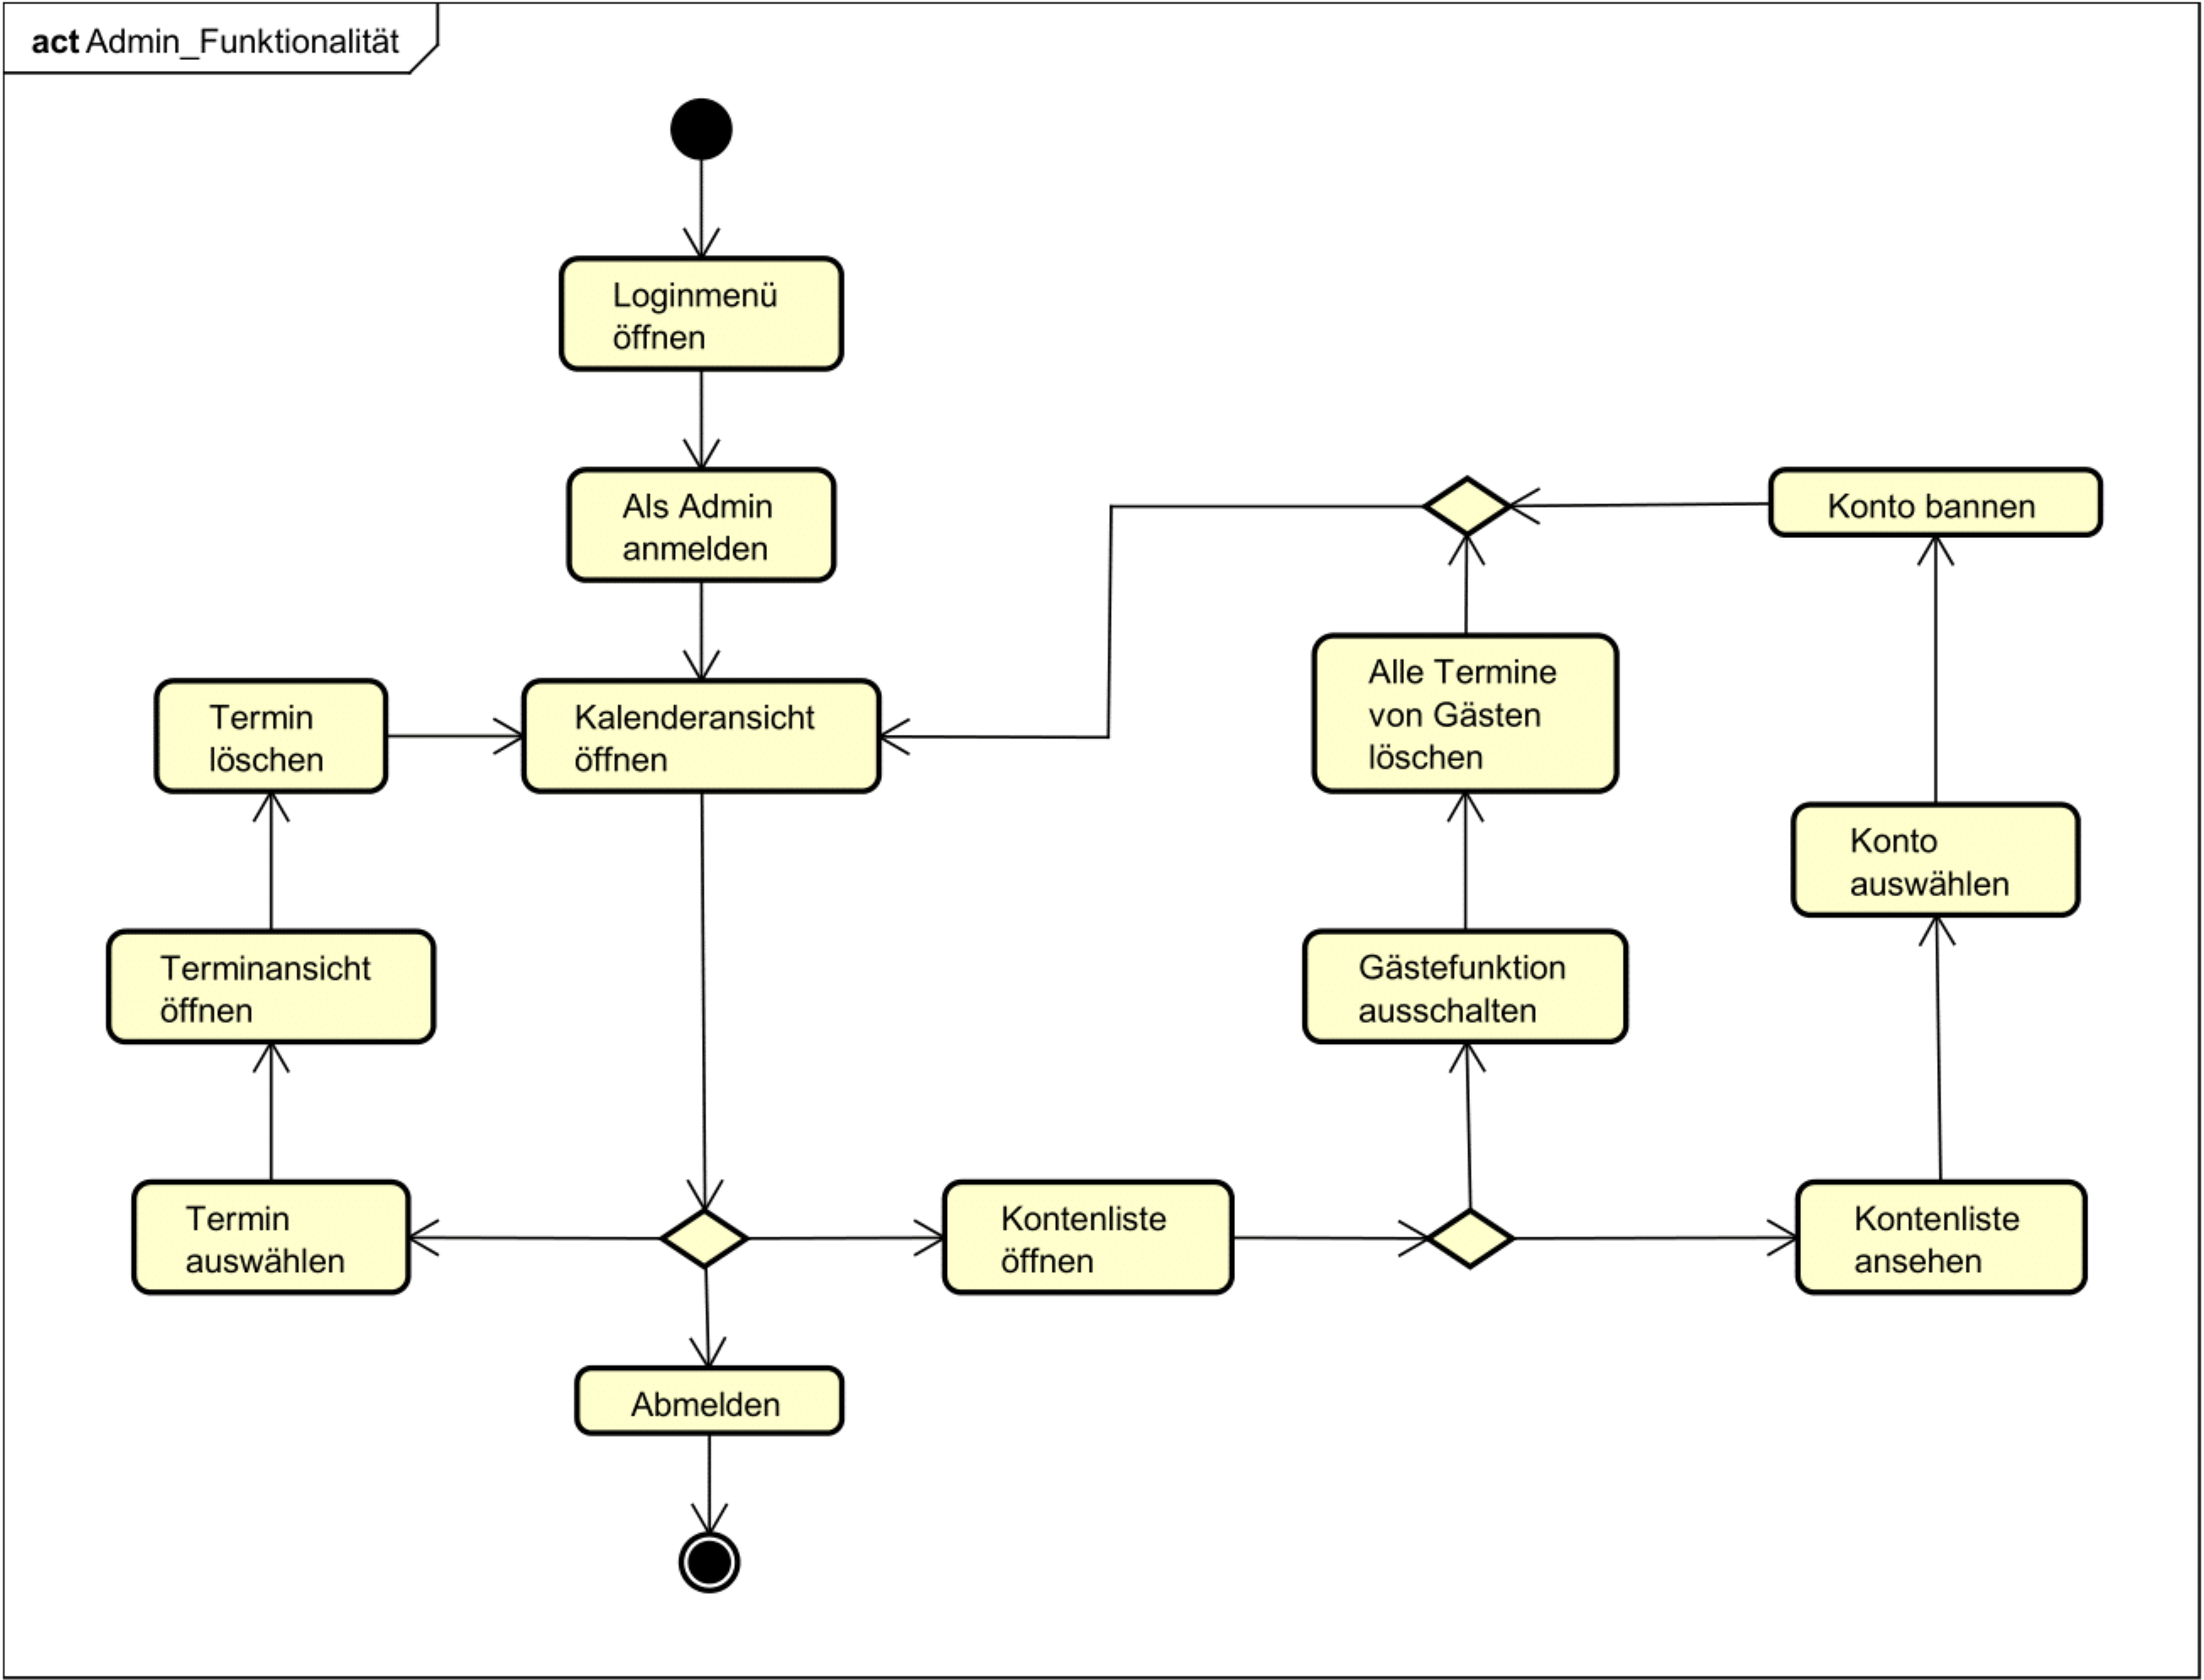
\includegraphics[width=\textwidth]{figures/activitydiagrams/adminfunk}
    \caption{Aktivitätsdiagramm für die Admin-Funktionalität}
    \label{fig:activity_diagram_admin}
\end{figure}
\clearpage
\subsection{Anmeldeprozess}

In Abbildung \ref{fig:activity_diagram_login} ist das Aktivitätsdiagramm für den Anmeldeprozess dargestellt,
welches die Musskriterien \ref{MK2} und \ref{MK17} abdeckt, sowie die Produktfunktionen \ref{F20} und \ref{F100}.
\begin{figure}[ht]
    \centering
    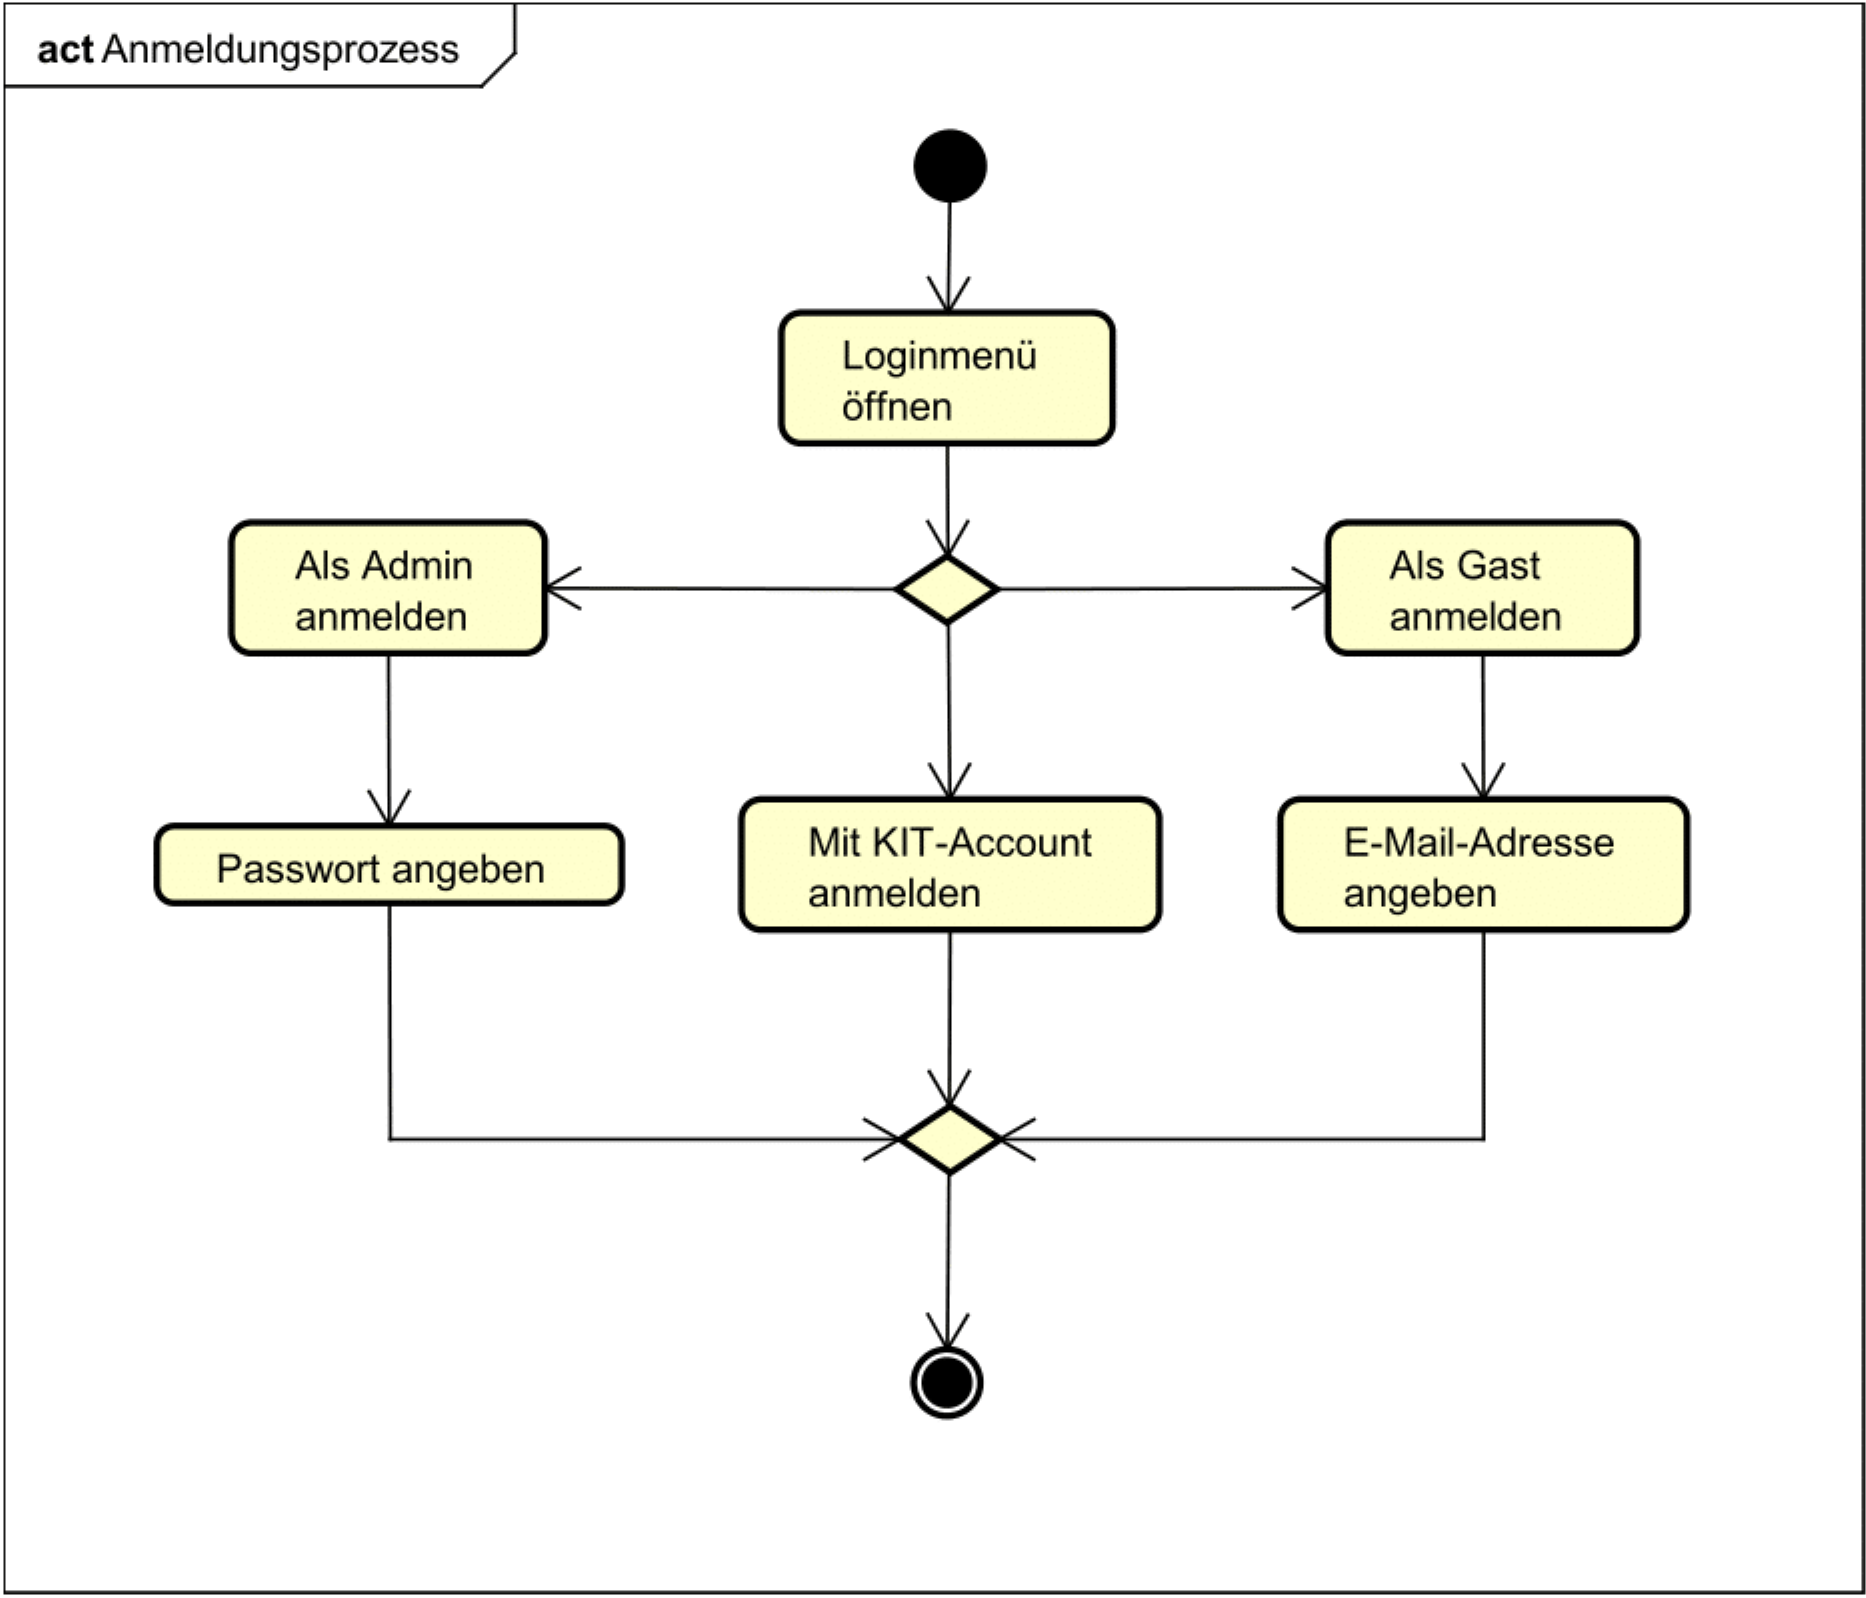
\includegraphics[width=\textwidth]{figures/activitydiagrams/anmeldeprozess}
    \caption{Aktivitätsdiagramm für den Anmeldeprozess}
    \label{fig:activity_diagram_login}
\end{figure}
\clearpage
\subsection{Termin erstellen}

In Abbildung \ref{fig:activity_diagram_booking} ist das Aktivitätsdiagramm für das Erstellen eines Termins dargestellt,
welches die Musskriterien \ref{MK2}, \ref{MK3}, \ref{MK5}, \ref{MK6}, \ref{MK9}, \ref{MK10}, \ref{MK12} und \ref{MK13} abdeckt,
sowie die Produktfunktionen \ref{F20}, \ref{F30} und \ref{F40}.
\begin{figure}[ht]
    \centering
    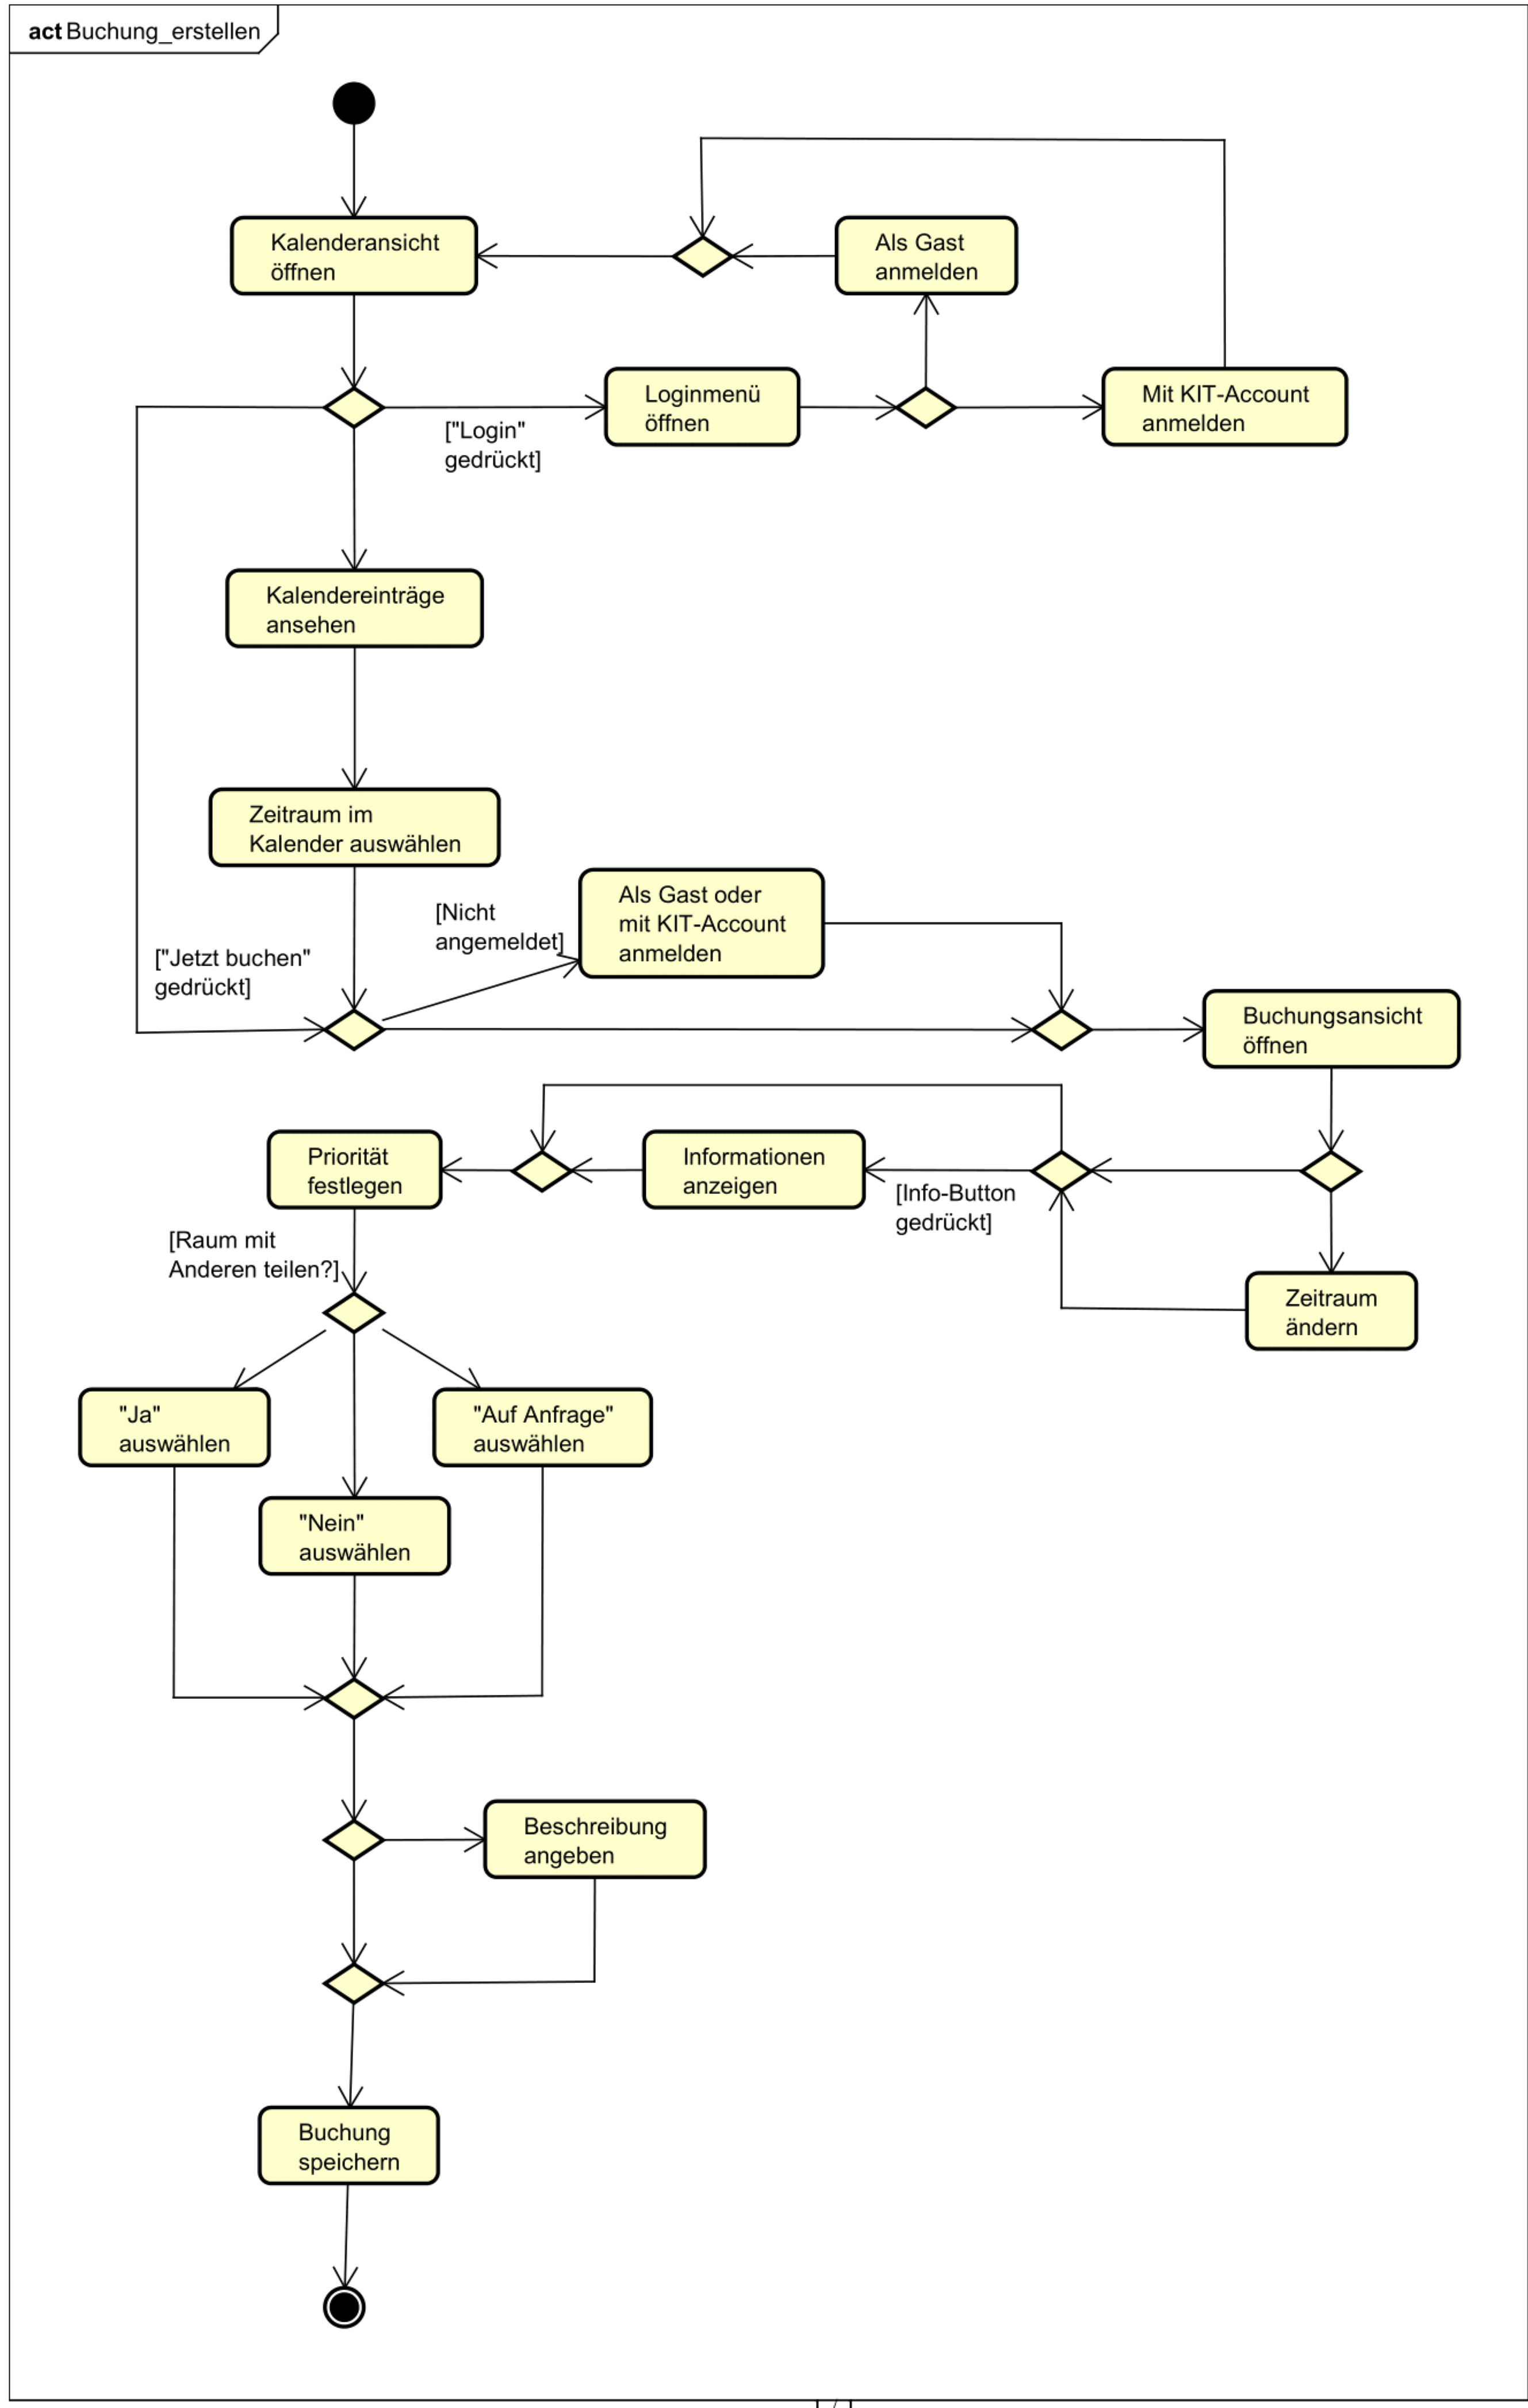
\includegraphics[width=0.7\textwidth]{figures/activitydiagrams/buchungerstellen}
    \caption{Aktivitätsdiagramm für das Erstellen eines Termins}
    \label{fig:activity_diagram_booking}
\end{figure}


\clearpage
\subsection{Termine verwalten}
In Abbildung \ref{fig:activity_diagram_booking_manage} ist das Aktivitätsdiagramm für das Verwalten von Terminen dargestellt,
welches die Musskriterien \ref{MK2}, \ref{MK11} und \ref{MK16} abdeckt, sowie die Produktfunktionen \ref{F20} und \ref{F90}.
\begin{figure}[ht]
    \centering
    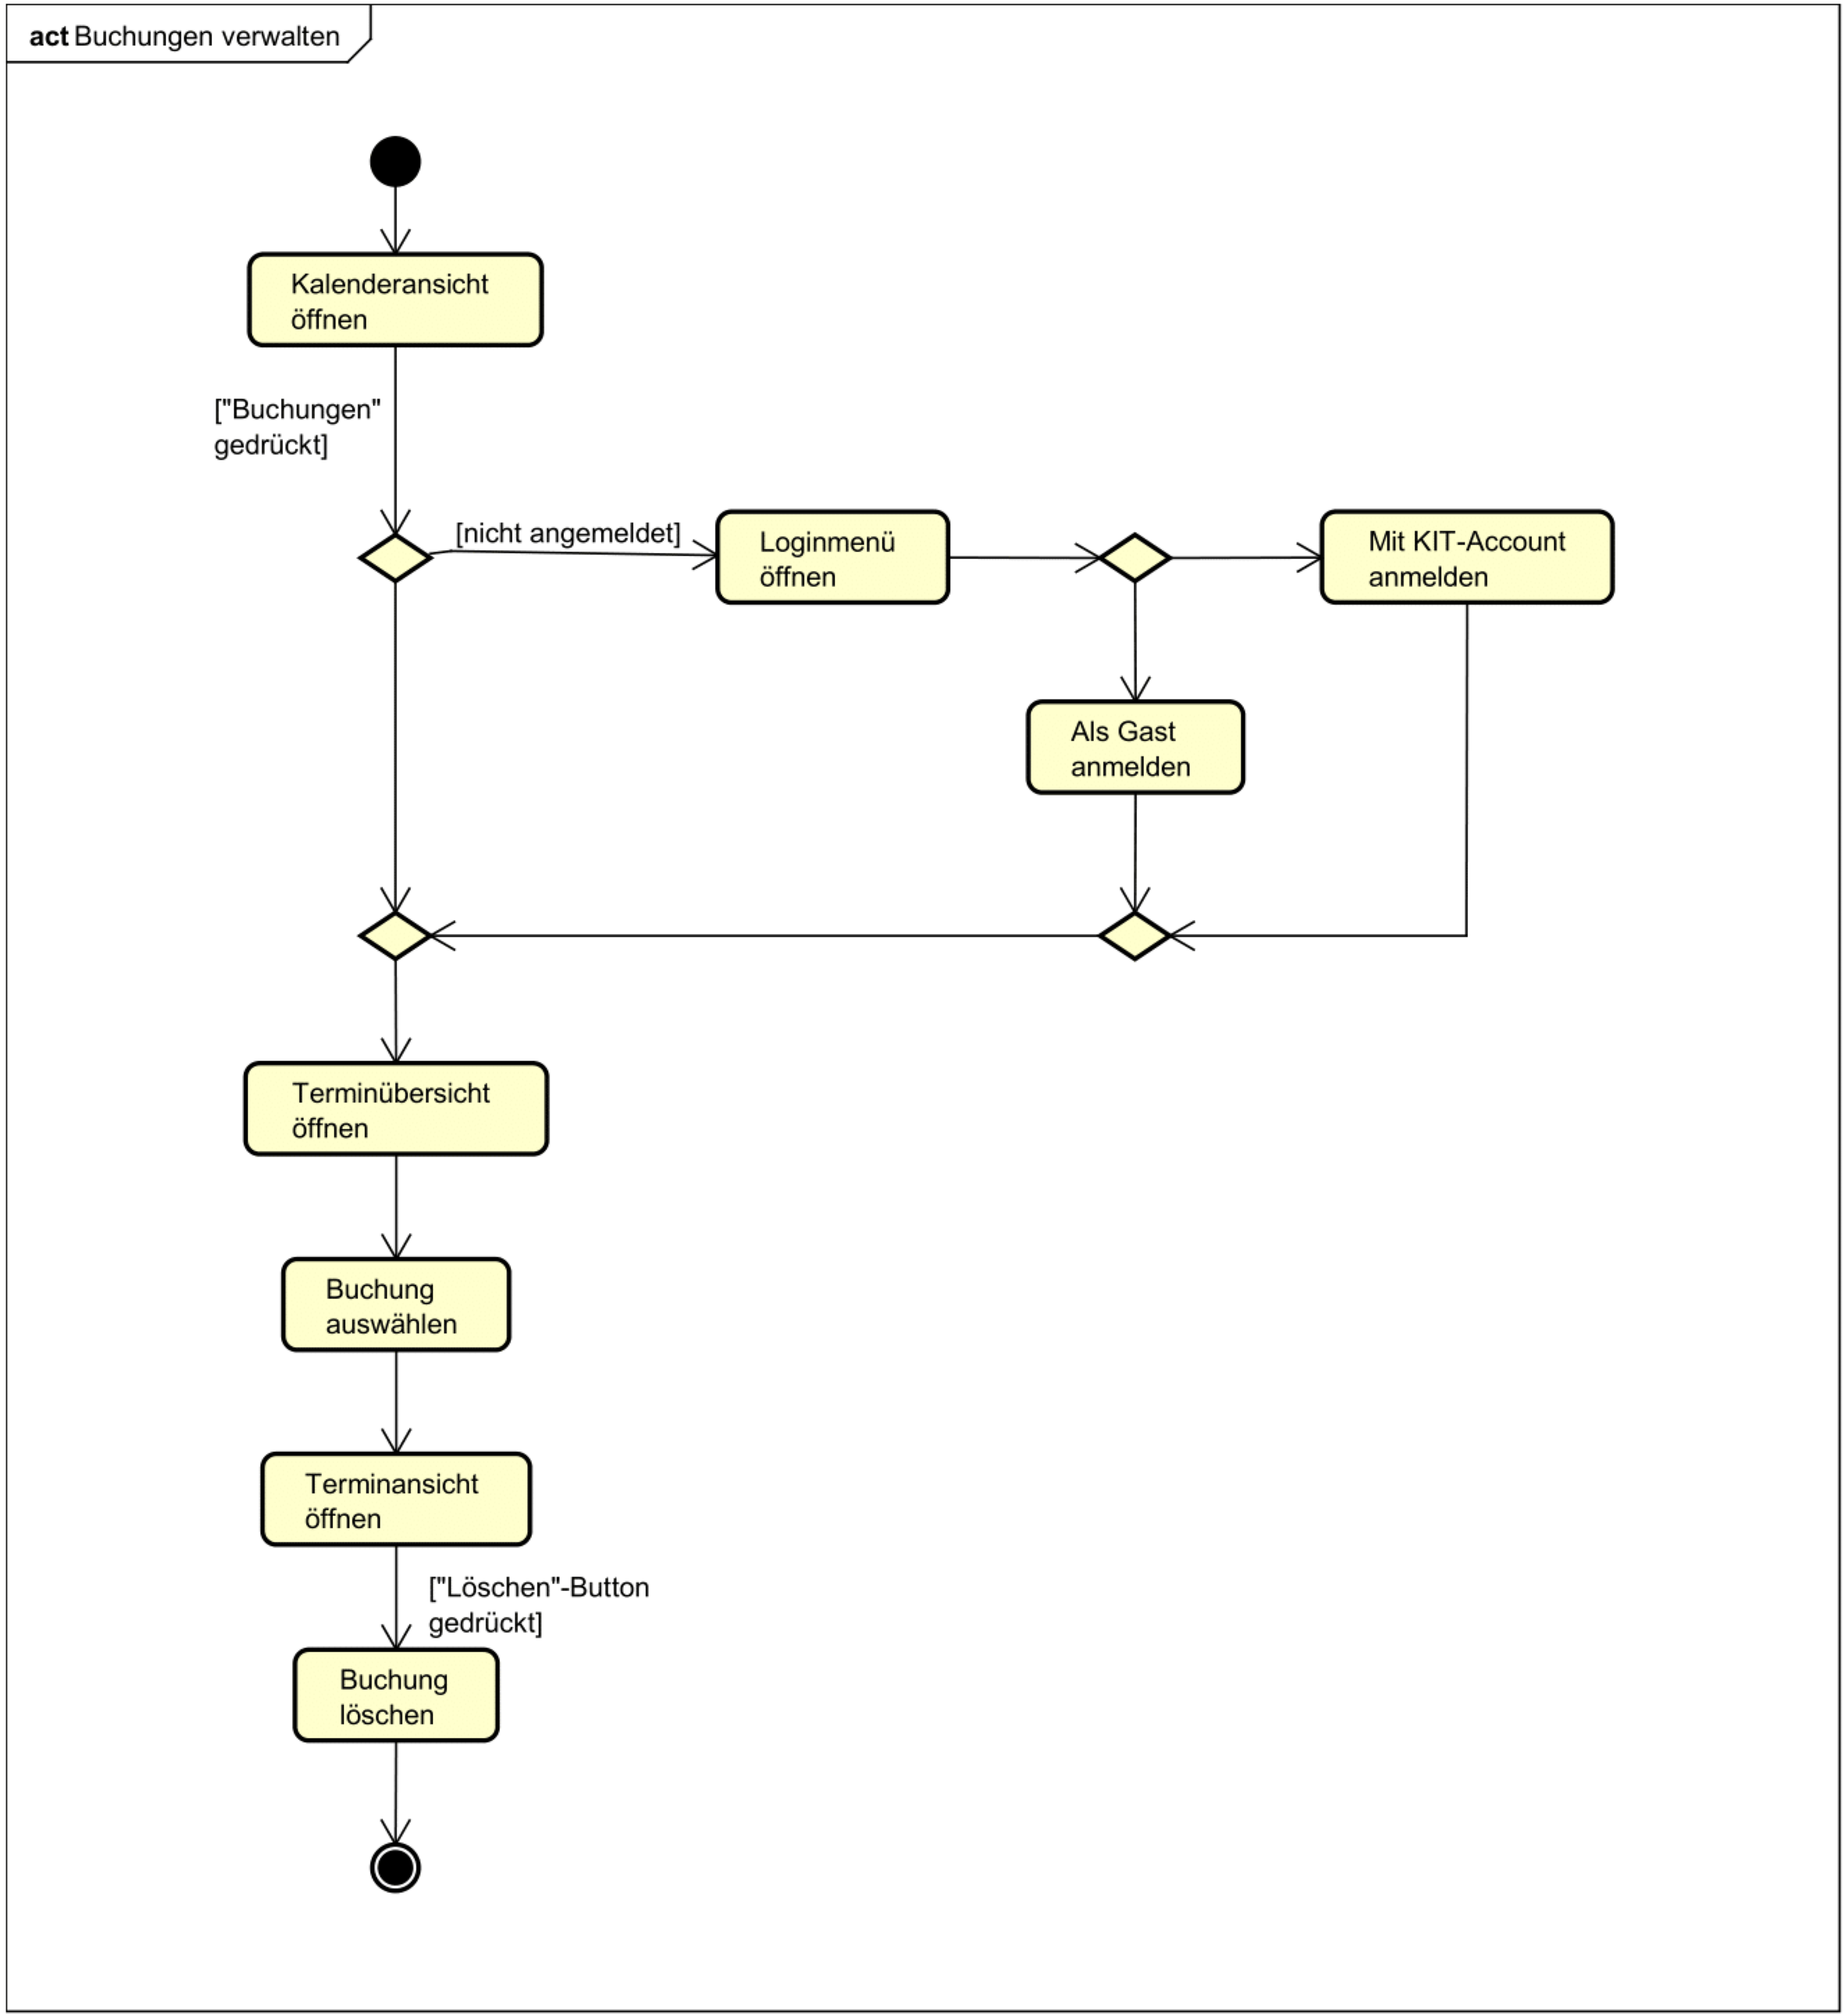
\includegraphics[width=0.8\textwidth]{figures/activitydiagrams/buchungverwalten}
    \caption{Aktivitätsdiagramm für das Verwalten von Terminen}
    \label{fig:activity_diagram_booking_manage}
\end{figure}

\clearpage
\subsection{Termin Ansicht}
In Abbildung \ref{fig:activity_diagram_calendar} ist das Aktivitätsdiagramm für die Ansicht \textit{Termin} dargestellt,
welches die Musskriterien \ref{MK2}, \ref{MK5}, \ref{MK8}, \ref{MK16}, \ref{MK17} und \ref{MK19} abdeckt,
sowie die Produktfunktionen \ref{F20}, \ref{F50}, \ref{F90}, \ref{F100} und \ref{F130}.
\begin{figure}[ht]
    \centering
    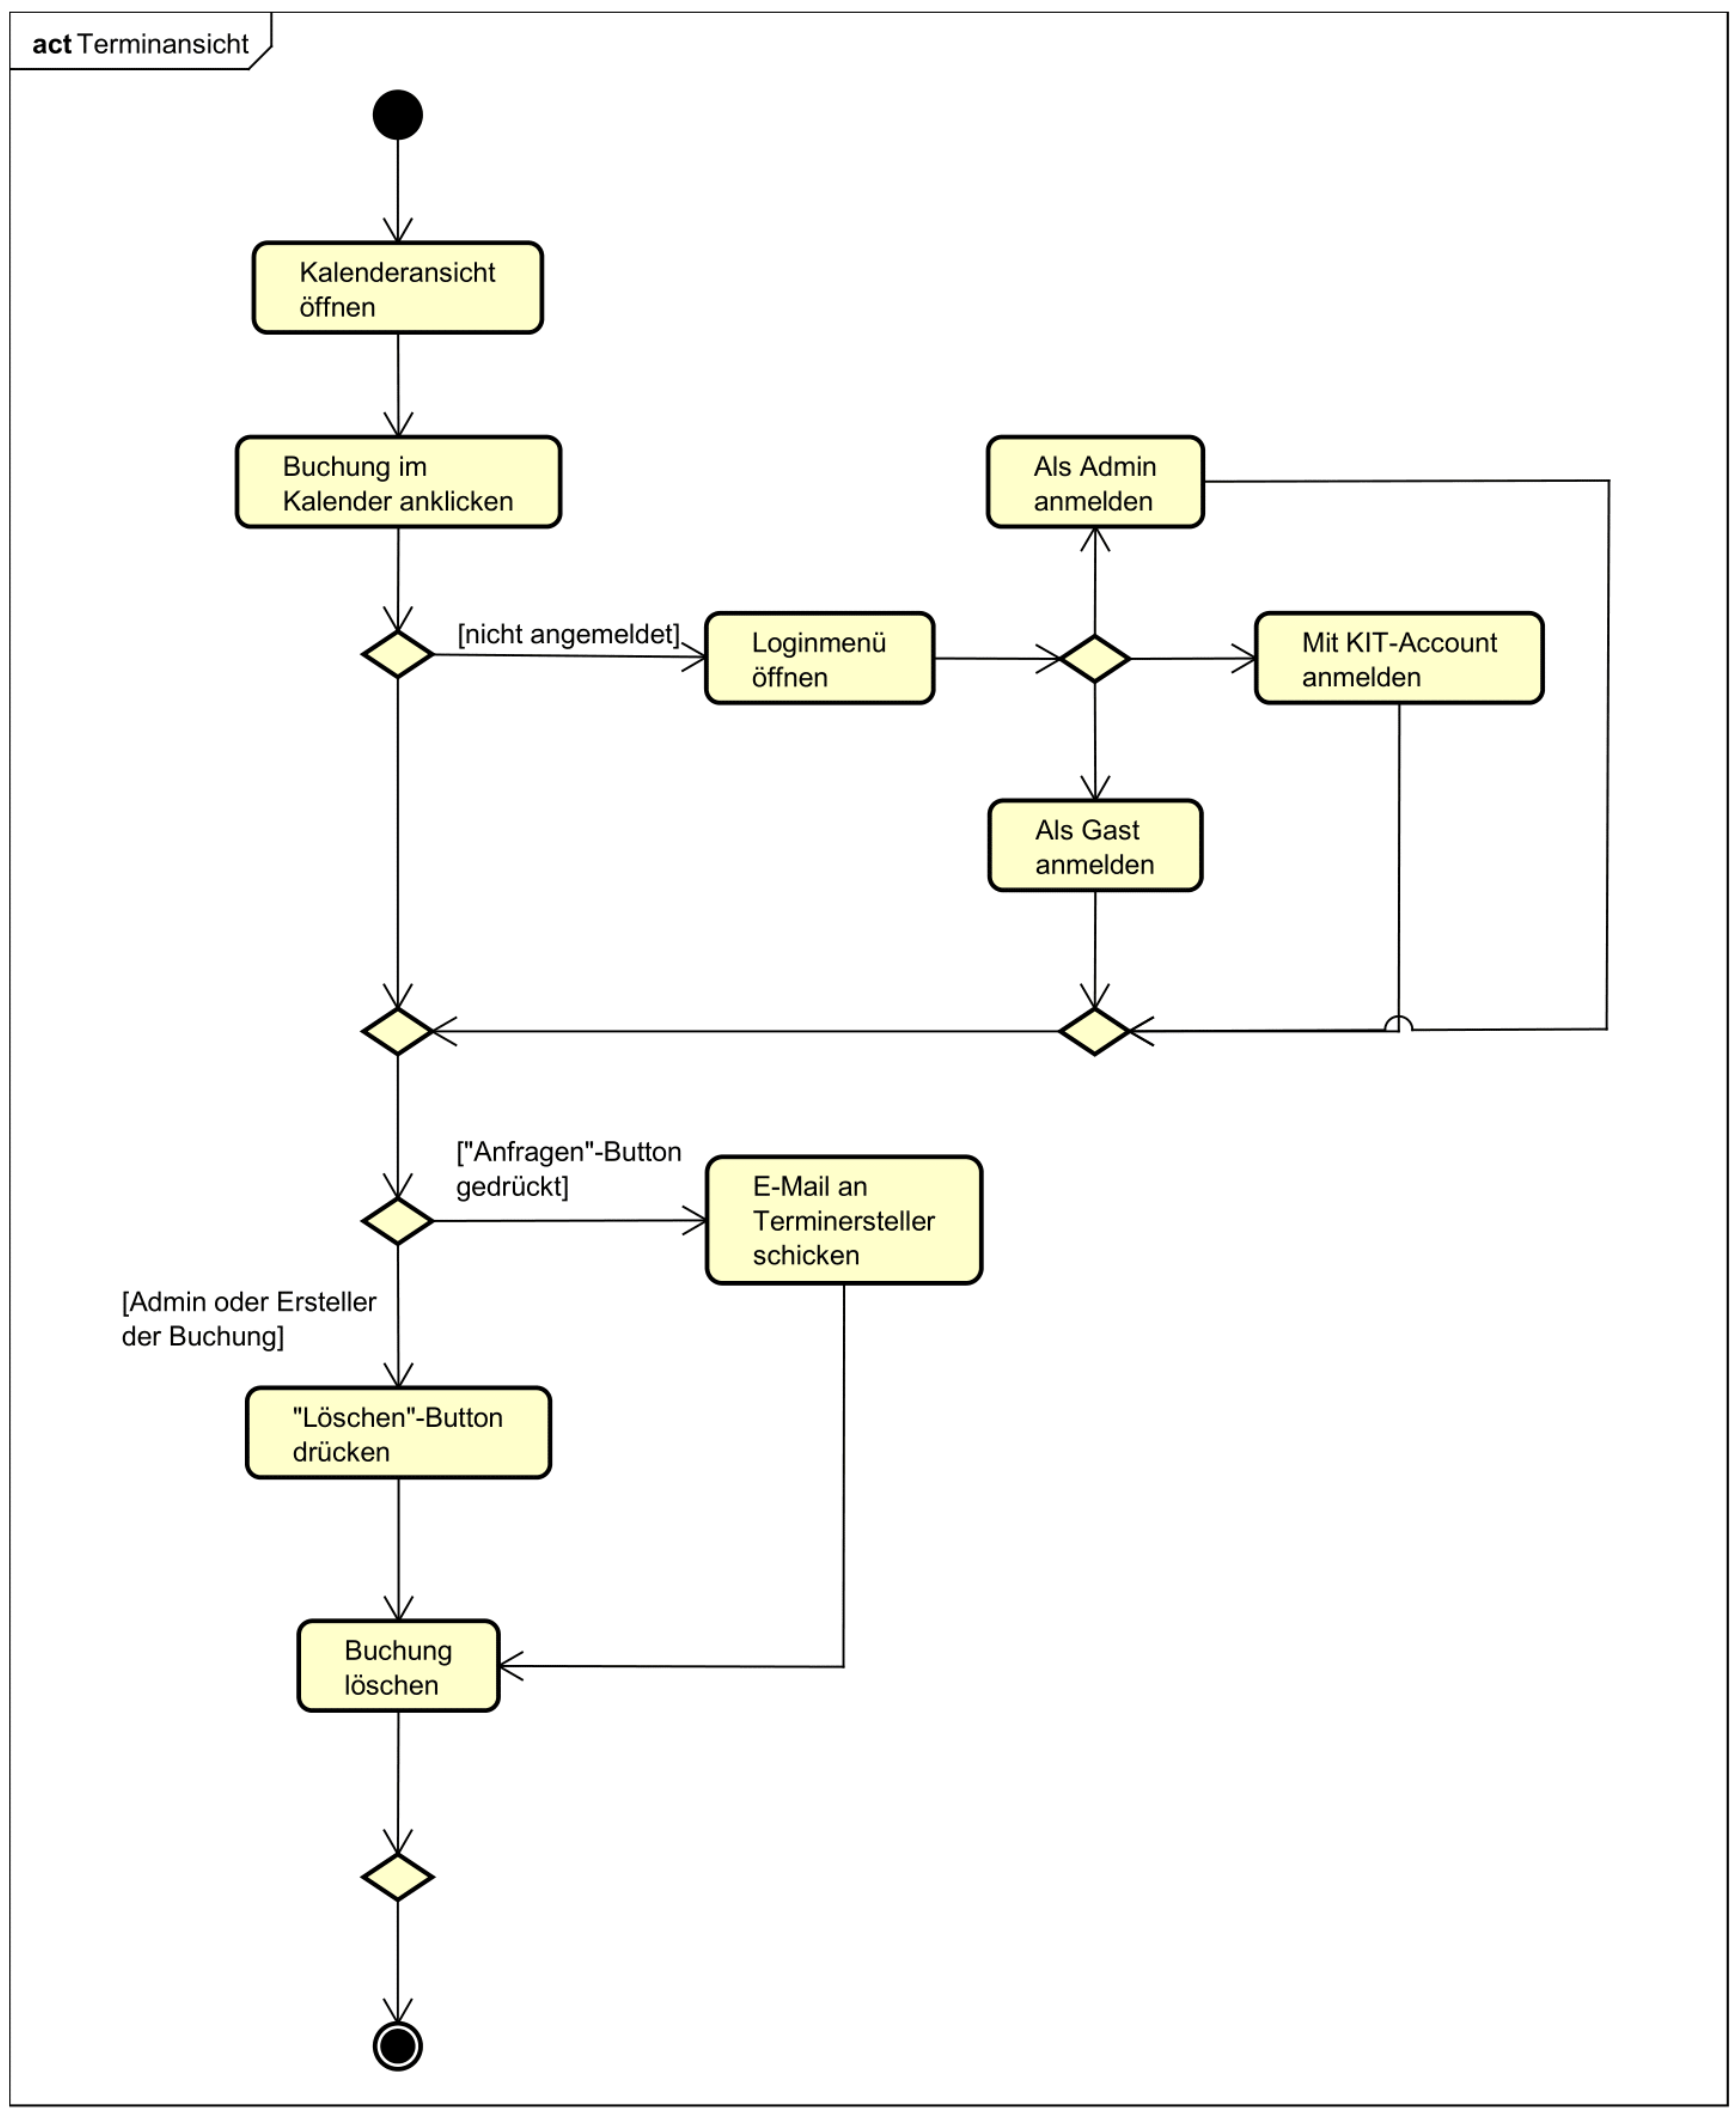
\includegraphics[width=0.8\textwidth]{figures/activitydiagrams/terminansicht}
    \caption{Aktivitätsdiagramm für die Ansicht \textit{Termin}}
    \label{fig:activity_diagram_calendar}
\end{figure}
%!TEX root = ../Pflichtenheft.tex

% Kapitel 4
%-------------------------------------------------------------------------------

\chapter{Produktfunktionen}
\label{chap:product_functions}


\section{Unangemeldete Nutzende}\label{sec:unangemeldete-benutzer-funktionen}

\begin{table}[htbp]
    \centering
    \begin{tabularx}{\textwidth}{ l|X|>{\raggedright\arraybackslash}X }
        \textbf{Nr.} & \textbf{Funktion} & \textbf{Kriterien} \\ \hline\hline
        \ref{F10} & Startseite besuchen &~\ref{MK1}, ~\ref{MK4}, ~\ref{WK1} \\
        \ref{F20} & Login &~\ref{MK2}, ~\ref{MK4} \\
        \ref{F70} & Anzeige des Raumstatus &~\ref{MK18} \\
    \end{tabularx}
    \caption{Überblick von Funktionen für unangemeldete Nutzende.}
    \label{tab:non_loggedin_functions}
\end{table}


\section{Angemeldete Nutzende}\label{sec:angemeldete-benutzer-funktionen}
\begin{table}[htbp]
    \centering
    \begin{tabularx}{\textwidth}{ l|X|>{\raggedright\arraybackslash}X }
        \textbf{Nr.} & \textbf{Funktion} & \textbf{Kriterien} \\ \hline\hline
        \ref{F10} & Startseite besuchen &~\ref{MK1}, ~\ref{MK4}, ~\ref{WK1} \\
        \ref{F100} & Login mit Adminkonto &~\ref{MK17} \\
        \ref{F30} & Abmelden &~\ref{MK3}, ~\ref{MK4} \\
        \ref{F40} & Reservieren &~\ref{MK9}, ~\ref{MK10}, ~\ref{MK12}, ~\ref{MK13}, ~\ref{MK14}, ~\ref{WK4}, ~\ref{WK11} \\
        \ref{F70} & Benachrichtigung &~\ref{WK10} \\
        \ref{F80} & Anzeige des Raumstatus &~\ref{MK20} \\
        \ref{F90} & Stornierung einer Reservierung &~\ref{MK16} \\
        \ref{F130} & Terminkonfliktauflösung &~\ref{MK14} \\
    \end{tabularx}
    \caption{Überblick von Funktionen für angemeldete Nutzende.}
    \label{tab:loggedin_functions}
\end{table}
\newpage
\section{Administrator*innen}\label{sec:adminfunktionen}

\begin{table}[htbp]
    \centering
    \begin{tabularx}{\textwidth}{ l|X|>{\raggedright\arraybackslash}X  }
        \textbf{Nr.} & \textbf{Funktion} & \textbf{Kriterien} \\ \hline\hline
        \ref{F10} & Startseite besuchen &~\ref{MK1}, ~\ref{MK4}, ~\ref{WK1} \\
        \ref{F30} & Abmelden &~\ref{MK3}, ~\ref{MK4} \\
        \ref{F40} & Reservieren &~\ref{MK9}, ~\ref{MK10}, ~\ref{MK12}, ~\ref{MK13}, ~\ref{MK14}, ~\ref{WK4}, ~\ref{WK11} \\
        \ref{F50} & Löschen von Terminen durch Administratoren &~\ref{MK18} \\
        \ref{F60} & Deaktivierung von Konten &~\ref{MK19} \\
        \ref{F70} & Benachrichtigung bei freiem Raum &~\ref{WK10} \\
        \ref{F80} & Anzeige des Raumstatus &~\ref{MK20} \\
        \ref{F90} & Stornierung einer Reservierung &~\ref{MK16} \\
        \ref{F100} & Anmelden als Admin &~\ref{MK17} \\
        \ref{F110} & Deaktivieren von Gastkonto-Anmeldung &~\ref{MK18} \\
        \ref{F120} & Öffnungszeiten einstellen &~\ref{MK21} \\
        \ref{F130} & Terminkonfliktauflösung &~\ref{MK14} \\
    \end{tabularx}
    \caption{Überblick von Funktionen für Admins.}
    \label{tab:adminfunctions}
\end{table}



\begin{function}{10}{Startseite}
    \item[Anwendungsfall:] Initiales besuchen der Webseite
    \item[Anforderung:]~\ref{MK1}, ~\ref{MK4}, ~\ref{WK1}
    \item[Ziel:] Den Nutzenden wird ohne Anmeldung die Ansicht \textit{Kalender} gezeigt.
    \item[Vorbedingung:] Die Nutzenden haben eine Internetverbindung und im \gls{Browser}~die Webseite geöffnet.
    \item[Nachbedingung Erfolg:] Die Nutzenden sehen die Ansicht \textit{Kalender} mit zukünftigen Reservierungen.
    \item[Nachbedingung Fehlschlag:] Die Nutzenden sind nicht in der Lage mit der Webseite weiter zu interagieren.
    \item[Auslösendes Ereignis:] Die Nutzenden verwenden ihre \gls{Browser}~, um die Webseite aufzurufen.
    \item[Beschreibung:]~
    \begin{enumerate}
        \item Die Nutzenden navigieren in ihren Browsern auf die Webseite.
        \item Die Startseite lädt und zeigt den Nutzenden die Ansicht \textit{Kalender} an.
    \end{enumerate}
    \item[Erweiterung:] Sollte es mehr als ein Arbeitsraum geben, so sollte hier vom Nutzenden die Auswahl getroffen werden, bevor die Ansicht \textit{Kalender} angezeigt wird.
\end{function}

\pagebreak

\begin{function}{20}{Anmelden}
    \item[Anwendungsfall:] Anmelden bzw.\ Registrieren
    \item[Anforderung:]~\ref{MK2}, ~\ref{MK4}
    \item[Ziel:] Die Nutzenden können sich mit ihren KIT-Konten oder lokalen Gastkonten anmelden.
    \item[Vorbedingung:] Die Nutzenden haben eine Internetverbindung und die Anwendung ist gestartet.
    \item[Nachbedingung Erfolg:] Die Nutzenden sind angemeldet und können Ereignisse ansehen und bearbeiten.
    \item[Nachbedingung Fehlschlag:] Die Nutzenden sind nicht angemeldet und können keine Ereignisse ansehen oder bearbeiten.
    \item[Auslösendes Ereignis:] Die Nutzenden öffnen die Anwendung und versuchen, einem Termin zu erstellen oder mit einem bereits existierenden Termin zu interagieren.
    \item[Beschreibung:] ~
    \begin{enumerate}
        \item Die Nutzenden wählen in einem Dialog die Anmeldemethode aus.
        \item Sollten diese noch keinen Account haben, so wird statt eine Anmeldung eine Registrierung vollzogen.
        \item Die Nutzenden werden, falls nötig, auf die KIT-Login-Seite weitergeleitet.
        \item Falls keine lokale Gast-Anmeldung gewählt wurde, geben die Nutzenden ihre Zugangsdaten ein.
        \item Die Anwendung überprüft die Zugangsdaten und meldet die Nutzenden an.
        \item Bei einer Gast-Anmeldung wird zusätzlich noch eine E-Mail hinterlegt.
        \item Die Nutzenden werden zur nächsten Seite weitergeleitet.
    \end{enumerate}
\end{function}

\pagebreak

\begin{function}{30}{Abmelden}
    \item[Anwendungsfall:] Abmelden
    \item[Anforderung:]~\ref{MK3}
    \item[Ziel:] Die Nutzenden können sich von der Anwendung abmelden.
    \item[Vorbedingung:] Der/die Nutzende ist angemeldet.
    \item[Nachbedingung Erfolg:] Der/die Nutzende ist abgemeldet und wird auf die Startseite weitergeleitet.
    \item[Nachbedingung Fehlschlag:] Der/die Nutzende ist nicht abgemeldet und erhält eine Fehlermeldung.
    \item[Auslösendes Ereignis:] Die/der Nutzende wählt die Option zum Abmelden aus.
    \begin{enumerate}
        \item Der/die Nutzende wählt die Funktion zum Abmelden aus.
        \item Der/die Nutzende wird abgemeldet und auf die Startseite weitergeleitet.
    \end{enumerate}
\end{function}


\pagebreak

\begin{function}{40}{Reservierung}
    \item[Anwendungsfall:] Reservierung
    \item[Anforderung:]~\ref{MK9} und~\ref{MK10}, ~\ref{MK12}, ~\ref{MK13}, ~\ref{MK14}, ~\ref{WK4} und~\ref{WK11}
    \item[Ziel:] Die nutzende Person kann einen Raum reservieren.
    \item[Vorbedingung:] Die nutzende Person ist angemeldet und in der Ansicht \textit{Kalender}.
    \item[Nachbedingung Erfolg:] Eine Reservierung wird gespeichert und die nutzende Person zur Ansicht \textit{Termin} weitergeleitet.
    \item[Nachbedingung Fehlschlag:] Die Reservierung wird nicht gespeichert und die nutzende Person erhält eine Fehlermeldung.
    \item[Auslösendes Ereignis:] Die nutzende Person wählt einen Startzeitpunkt.
    \item[Beschreibung:] ~
    \begin{enumerate}
        \item Die nutzende Person wählt einen Start- und Endzeitpunkt auf 15 minuten genau und kann diese gegebenenfalls anpassen.
        \item Die nutzende Person gibt optional eine Beschreibung an.
        \item Die nutzende Person gibt an, ob sie bereit ist, den Raum mit weiteren zu teilen.
        \item Die nutzende Person wählt eine Prioritätsstufe.
        \item Die nutzende Person bestätigt ihre Eingaben.
        \item Die Anwendung prüft, ob der Raum in dem Zeitraum verfügbar ist.
        \item Ist dies der Fall, wird die Reservierung gespeichert und die nutzende Person zur Ansicht \textit{Kalender} weitergeleitet.
        Wenn nötig, wird eine E-Mail an die Ersteller*innen überschriebener Reservierungen gesendet.
        \item Die Anwendung überprüft, ob die angegebene Priorität andere Termine beeinflusst und löst konflikte entsprechend.~(siehe~\ref{F130})
        \item Der nutzenden Person wird dieser Konflikt mitgeteilt und sobald dieser geklärt, wird den beteiligten Parteien der entschluss via E-Mail mitgeteilt.
    \end{enumerate}
    \item[Erweiterung:] ~
    \begin{enumerate}
        \item Nach dem Erstellen des Termins könnte dieser als iCal-Export zur verfügung gestellt werden.
        \item Durch einen zusätzlichen Quick-Checkin-Button könnte dieser Prozess simpler und kürzer gemacht werden.
    \end{enumerate}
\end{function}

\pagebreak

\begin{function}{50}{Löschen von Terminen durch das Adminkonto}
    \item[Anwendungsfall:] Löschen von Terminen durch das Adminkonto
    \item[Anforderung:] ~\ref{MK19}
    \item[Ziel:] Ein/e Administrator*in kann bestehende Termine löschen.
    \item[Vorbedingung:] Ein/e Administrator*in ist angemeldet und die Ansicht \textit{Kalender} wird angezeigt.
    \item[Nachbedingung Erfolg:] Der Termin wird aus dem System entfernt und der/die Administrator*in erhält eine Erfolgsmeldung.
    \item[Nachbedingung Fehlschlag:] Der Termin wird nicht gelöscht und der/die Administrator*in erhält eine Fehlermeldung.
    \item[Auslösendes Ereignis:] Ein/e Administrator*in wählt einen Termin aus, welcher gelöscht werden soll.
    \item[Beschreibung:] ~
    \begin{enumerate}
        \item Ein/e Administrator*in öffnet die Ansicht \textit{Kalender}.
        \item Der/die Administrator*in wählt den Termin aus, welcher gelöscht werden soll.
        \item Der/die Administrator*in wird gefragt, ob es den Termin wirklich löschen möchte (Bestätigungsabfrage).
        \item Falls der/die Administrator*in bestätigt, wird der Termin gelöscht.
        \item Eine Bestätigungsmeldung wird angezeigt (z.B.\ `Termin erfolgreich gelöscht').
    \end{enumerate}
\end{function}

\pagebreak

\begin{function}{60}{Deaktivierung von Konten}
    \item[Anwendungsfall:] Deaktivierung von Konten
    \item[Anforderung:] ~\ref{MK18}
    \item[Ziel:] Ein Konto wird vom Adminkonto gesperrt.
    \item[Vorbedingung:] Ein/e Administrator*in ist angemeldet und betrachtet die Ansicht \textit{Kontoliste}.
    \item[Nachbedingung Erfolg:] Das Konto wird deaktiviert und kann nicht mehr zum Anmelden verwendet werden.
    \item[Nachbedingung Fehlschlag:] Das Konto bleibt aktiv und der/die Administrator*in erhält eine Fehlermeldung.
    \item[Auslösendes Ereignis:] Der/die Administrator*in wählt ein Konto aus, welches deaktiviert werden soll.
    \item[Beschreibung:] ~
    \begin{enumerate}
        \item Ein/e Administrator*in öffnet die Liste der Konten (Ansicht \textit{Kontoliste}).
        \item Der/die Administrator*in wählt ein Konto aus, welches deaktiviert werden soll.
        \item Der/die Administrator*in bestätigt die Deaktivierung.
        \item Das Konto wird deaktiviert und aus der aktiven Liste entfernt.
        \item Eine Bestätigungsmeldung wird angezeigt (z.B.\ \textit{Konto erfolgreich deaktiviert}).
    \end{enumerate}
\end{function}

\pagebreak

\begin{function}{70}{Benachrichtigung bei freiem Raum}
    \item[Anwendungsfall:] Benachrichtigung über freigewordenen Raum
    \item[Anforderung:] ~\ref{WK10}
    \item[Ziel:] Die Anwendung informiert Nutzende, wenn ein Raum wieder frei wird.
    \item[Vorbedingung:] Die Nutzenden haben sich für den Raum interessiert und haben eine Benachrichtigung angefordert.
    \item[Nachbedingung Erfolg:] Die Nutzenden werden über die Freigabe des Raums per E-Mail oder Benachrichtigung informiert.
    \item[Nachbedingung Fehlschlag:] Die Nutzenden erhalten keine Benachrichtigung, und eine Fehlermeldung wird angezeigt.
    \item[Auslösendes Ereignis:] Der Raum wird freigegeben, nachdem eine vorherige Reservierung aufgehoben oder geändert wurde.
    \item[Beschreibung:] ~
    \begin{enumerate}
        \item Die Nutzenden wählen aus, ob sie für den Raum Benachrichtigungen erhalten möchten, wenn er wieder frei wird.
        \item Sobald der Raum wieder verfügbar ist, prüft das System, ob die nutzende Person für den Raum eine Benachrichtigung angefordert haben.
        \item Den betroffenen Nutzenden wird eine E-Mail oder Benachrichtigung zugeschickt, dass der Raum nun wieder verfügbar ist.
    \end{enumerate}
\end{function}

\pagebreak

\begin{function}{80}{Anzeige des Raumstatus}
    \item[Anwendungsfall:] Anzeige des Raumstatus
    \item[Anforderung:] ~\ref{MK20} \ref{WK9}
    \item[Ziel:] Die Anwendung stellt den Raumstatus, einschließlich der aktuellen Belegung und Priorität, übersichtlich dar.
    \item[Vorbedingung:] Die Nutzenden sind auf der Ansicht \textit{Kalender} und müssen nicht angemeldet sein.
    \item[Nachbedingung Erfolg:] Der Raumstatus wird auf einer öffentlichen Seite korrekt angezeigt, inklusive Belegung und Priorität (z.B.\ durch farbige Banner).
    \item[Nachbedingung Fehlschlag:] Der Raumstatus wird nicht angezeigt oder ist unvollständig.
    \item[Auslösendes Ereignis:] Die Nutzenden öffnen die Ansicht \textit{Kalender}.
    \item[Beschreibung:] ~
    \begin{enumerate}
        \item Die Nutzenden öffnen die Seite.
        \item Die Belegung des Raumes wird mit dem entsprechenden Status angezeigt, der die aktuelle Belegung widerspiegelt.
        \item Falls der Raum belegt ist, wird dies deutlich sichtbar gemacht (z.B.\ durch ein Banner oder ein entsprechendes Symbol).
        \item Dabei wird die Priorität klar dargestellt.
        \item Der Raumstatus ist für alle Nutzenden sichtbar, ohne dass eine Anmeldung erforderlich ist.
    \end{enumerate}
\end{function}

\pagebreak

\begin{function}{90}{Stornierung einer Reservierung}
    \item[Anwendungsfall:] Stornierung einer Reservierung
    \item[Anforderung:] ~\ref{MK16}
    \item[Ziel:] Die Nutzenden können eine bestehende Reservierung stornieren.
    \item[Vorbedingung:] Die Nutzenden sind angemeldet und haben eine aktive Reservierung.
    \item[Nachbedingung Erfolg:] Die Reservierung wird storniert und die Nutzenden erhalten eine Erfolgsmeldung.
    \item[Nachbedingung Fehlschlag:] Die Reservierung wird nicht storniert und die Nutzenden erhalten eine Fehlermeldung.
    \item[Auslösendes Ereignis:] Die Nutzenden wählen die Option zur Stornierung einer bestehenden Reservierung.
    \item[Beschreibung:] ~
    \begin{enumerate}
        \item Die Nutzenden öffnen die Seite mit ihren aktuellen Reservierungen.
        \item Die Nutzenden wählen die Reservierung aus, die sie stornieren möchten.
        \item Die Nutzenden bestätigen die Stornierung der Reservierung (z.B.\ durch Klick auf \textit{Reservierung stornieren}).
        \item Eine Bestätigungsabfrage erscheint, in der die Nutzenden die Stornierung bestätigen müssen.
        \item Falls die Nutzenden bestätigen, wird die Reservierung storniert.
        \item Das System aktualisiert die Raumverfügbarkeit und zeigt den Nutzenden eine Bestätigungsmeldung (z.B.\ \textit{Reservierung erfolgreich storniert}).
        \item Die Nutzenden erhalten ggf.\ eine E-Mail oder eine Benachrichtigung über die Stornierung (optional).
    \end{enumerate}
\end{function}

\pagebreak

\begin{function}{100}{Anmelden mit Adminkonto}
    \item[Anwendungsfall:] Anmelden mit Adminkonto
    \item[Anforderung:]~\ref{MK17}
    \item[Ziel:] Berechtigte Personen können sich mit Passwort authentifizieren um auf das Adminkonto zugreifen zu können.
    \item[Vorbedingung:] Die nutzende Person befindet sich unangemeldet auf der Startseite.
    \item[Nachbedingung Erfolg:] Der Admin ist angemeldet und auf administrative Funktionen zugreifen.
    \item[Nachbedingung Fehlschlag:] Die nutzende Person bleibt unangemeldet auf der Startseite.
    \item[Auslösendes Ereignis:] Die nutzende Person ist unangemeldet auf der Startseite und versucht sich als Admin anzumelden.
    \item[Beschreibung:] ~
    \begin{enumerate}
        \item Die nutzende Person wählt die Admin-Anmeldemethode aus.
        \item Die Person gibt das Admin passwort ein.
        \item Die Anwendung überprüft die Zugangsdaten und lässt die anmeldung zu oder lehnt ab.
        \item Der Admin ist eingeloggt und zeigt die Startseite an.
    \end{enumerate}
\end{function}

\pagebreak

\begin{function}{110}{Deaktivieren von Gastkonto-Anmeldung}
    \item[Anwendungsfall:] Deaktivieren von Gastkonto-Anmeldung
    \item[Anforderung:]~\ref{MK18}
    \item[Ziel:] Die Anmeldung von Gastkonten wird deaktiviert.
    \item[Vorbedingung:] Ein/e Administrator*in ist angemeldet und die Ansicht \textit{Kontoliste} geöffnet.
    \item[Nachbedingung Erfolg:] Gastkonten können sich nicht mehr anmelden oder registrieren.
    \item[Nachbedingung Fehlschlag:] Gastkonten können sich immer noch anmelden, als auch registrieren.
    \item[Auslösendes Ereignis:] Die als Admin angemeldete Person wählt die Schaltfläche \textit{Gastkonto-Anmeldung deaktivieren}.
    \item[Beschreibung:] ~
    \begin{enumerate}
        \item Die Person wählt die Schaltfläche \textit{Gastkonto-Anmeldung deaktivieren} aus.
        \item Die Gastkonto-Anmeldung ist nun deaktiviert.
    \end{enumerate}
\end{function}

\pagebreak

\begin{function}{120}{Öffnungszeiten einstellen}
    \item[Anwendungsfall:] Öffnungszeiten einstellen
    \item[Anforderung:]~\ref{MK21}
    \item[Ziel:] Ein/e Administrator*in passt die Öffnungszeiten an.
    \item[Vorbedingung:] Der/die Administrator*in ist angemeldet und die Ansicht \textit{Kalender} geöffnet.
    \item[Nachbedingung Erfolg:] Die Öffnungszeiten sind geändert.
    \item[Nachbedingung Fehlschlag:] Die Öffnungszeiten bleiben gleich.
    \item[Auslösendes Ereignis:] Die als Admin angemeldete Person wählt die Schaltfläche zum Ändern der Öffnungszeiten.
    \item[Beschreibung:] ~
    \begin{enumerate}
        \item Die als Admin eingeloggte Person ändert die Öffnungszeiten (bzw.\ Schließzeiten) für einen gewählten Wochentag.
    \end{enumerate}
\end{function}

\pagebreak

\begin{function}{130}{Terminkonfliktauflösung}
    \item[Anwendungsfall:] Terminkonfliktauflösung
    \item[Anforderung:]~\ref{MK14}
    \item[Ziel:] Die Anwendung löst Terminkonflikte automatisch.
    \item[Vorbedingung:] Durch die Überlappung von einem neu gebuchten Termin entsteht ein Konflikt mit einem bereits existierenden Termin.
    \item[Nachbedingung Erfolg:] Der Konflikt ist gelöst.
    \item[Nachbedingung Fehlschlag:] Der Konflikt ist nicht gelöst und der neue Termin kann nicht hinzugefügt werden.
    \item[Auslösendes Ereignis:] Ein neuer Termin wurde erstellt und überlappt mit einem weiteren.
    \item[Beschreibung:] ~
    \begin{enumerate}
        \item Nachdem ein Termin erstellt worden ist, wird überprüft ob dieser überlappungen mit anderen Terminen hat.
        \item Ist dies der Fall wird überprüft, ob diese Kriterien ein Überlappen der Termine erlauben.
        \item Dabei wird ggf.\ den betroffenen Personen welche einen Termin \textit{Auf Anfrage} gestellt haben per E-Mail die Entscheidung zum Ablehnen oder Annehmen gegeben.
        \item Der Termin wird als gültig oder nicht klassifiziert und die betroffenen Personen benachrichtigt.
    \end{enumerate}
\end{function}
%!TEX root = ../Pflichtenheft.tex

\chapter{Produktdaten}
\label{chap:product_data}

Die Anwendung verwendet den Server als zentralen Speicherort für alle Daten.
Die Daten werden in einer \gls{PostgreSQL}-Datenbank gespeichert.
Auf dem Client werden nur temporäre Daten gespeichert, die für die Funktionalität der Anwendung notwendig sind.


\subsection*{Clientdaten}
\begin{itemize}
    \item Anmeldungscookie (falls die anmeldung via Gastkonto ist).
          Diese laufen nach 30 Tagen ab.
    \item Zustand der Anwendung (z.B.\ aktuelle Seite, geöffnete Dialoge)
\end{itemize}

\subsection*{Serverdaten}
\begin{itemize}
    \item Daten der Nutzenden (dauerhaft gespeichert)
    \begin{itemize}
        \item Kontoname (oder \textit{Gast} für Gastkonto)
        \item E-Mail-Adresse
        \item OAuth- oder Cookie-Token
        \item Blockierungsstatus (wahr oder falsch)
    \end{itemize}
    \item Ereignisdaten (30 Tage nach dem Termin werden diese Daten anonymisiert)
    \begin{itemize}
        \item Start- und Endzeitpunkt (Datenbank native Zeitdarstellung)
        \item Beschreibung
        \item Raum
        \item Ersteller*in
        \item Priorität
        \item Kollaborationsmodus
        \item E-Mail-Adresse
    \end{itemize}
    \item Raumdaten (dauerhaft gespeichert)
    \begin{itemize}
        \item Raumname
        \item Öffnungszeiten
    \end{itemize}
\end{itemize}
%!TEX root = ../Pflichtenheft.tex

% Kapitel 6
%-------------------------------------------------------------------------------

\chapter{Nichtfunktionale Anforderungen}
\label{chap:non_functional_req}


\notfunctional{1}{Die Anwendung soll schnell und einfach bedienbar sein.}
\notfunctional{2}{Die Anwendung soll auf mobilen sowie Desktop-Endgeräten ohne Einschränkungen nutzbar sein.}
\notfunctional{3}{Die Anwendung soll in allen gängigen \gls{Browser}n lauffähig sein. Insbesondere beinhaltet dies Firefox und Chrome auf Desktop- und Android-Geräten und Safari auf iOS.}
\notfunctional{4}{Die Anonymität der Nutzenden soll so weit wie möglich gewährleistet werden.}
\notfunctional{5}{Die Anwendung soll in verschiedenen Sprachen dargestellt werden können, insbesondere Deutsch und Englisch.}
\notfunctional{6}{Für Nutzende mit Sehschwäche soll die Anwendung durch Kompatibilität mit Screenreadern und kontrastreiche Farbgebung gut bedienbar sein.}
\notfunctional{7}{Die Anwendung soll so weit wie sinnvoll möglich sich an den \gls{WCAG} Richtlinen orientieren.}
%!TEX root = ../Pflichtenheft.tex

\chapter{Benutzeroberfläche}
\label{chap:ui}

\section{Haupseite und Buchung}

Die Startseite der Anwendung ist in \ref{fig:startseite} dargestellt.
Auf dieser haben Nutzende die Möglichkeit, dem Raum zu buchen oder auf andere Ansichten zu wechseln.
Das Banner in allen Ansichten zeigt den aktuellen Raumstatus an.
Insbesondere wird dadurch die Priorität des aktuellen Termins mithilfe der Farbe des Banners angezeigt.

Rechts in dieser Ansicht befindet sich ein Kalender, der die aktuelle Woche und die Termine in diesem Zeitraum anzeigt.
Die Termine sind farblich nach Priorität gekennzeichnet, weitere Informationen können durch Klicken auf den Termin eingesehen werden.
Neben dieser Möglichkeit, den Raum zu buchen, gibt es je nach Anmeldungsstatus einen Anmelde- oder Abmeldebutton und einen separaten Buchungsbutton,
für die die Verwendung des Kalenders Probleme bereitet.
Falls zur Zeit der Verwendung ein Termin des Nutzenden stattfindet, wird ein Quick-Checkout Button angezeigt,
der es ermöglicht, den Raum schnell freizugeben.
Siehe dazu auch \ref{fig:checkout}.

\begin{figure}[ht]
    \centering
    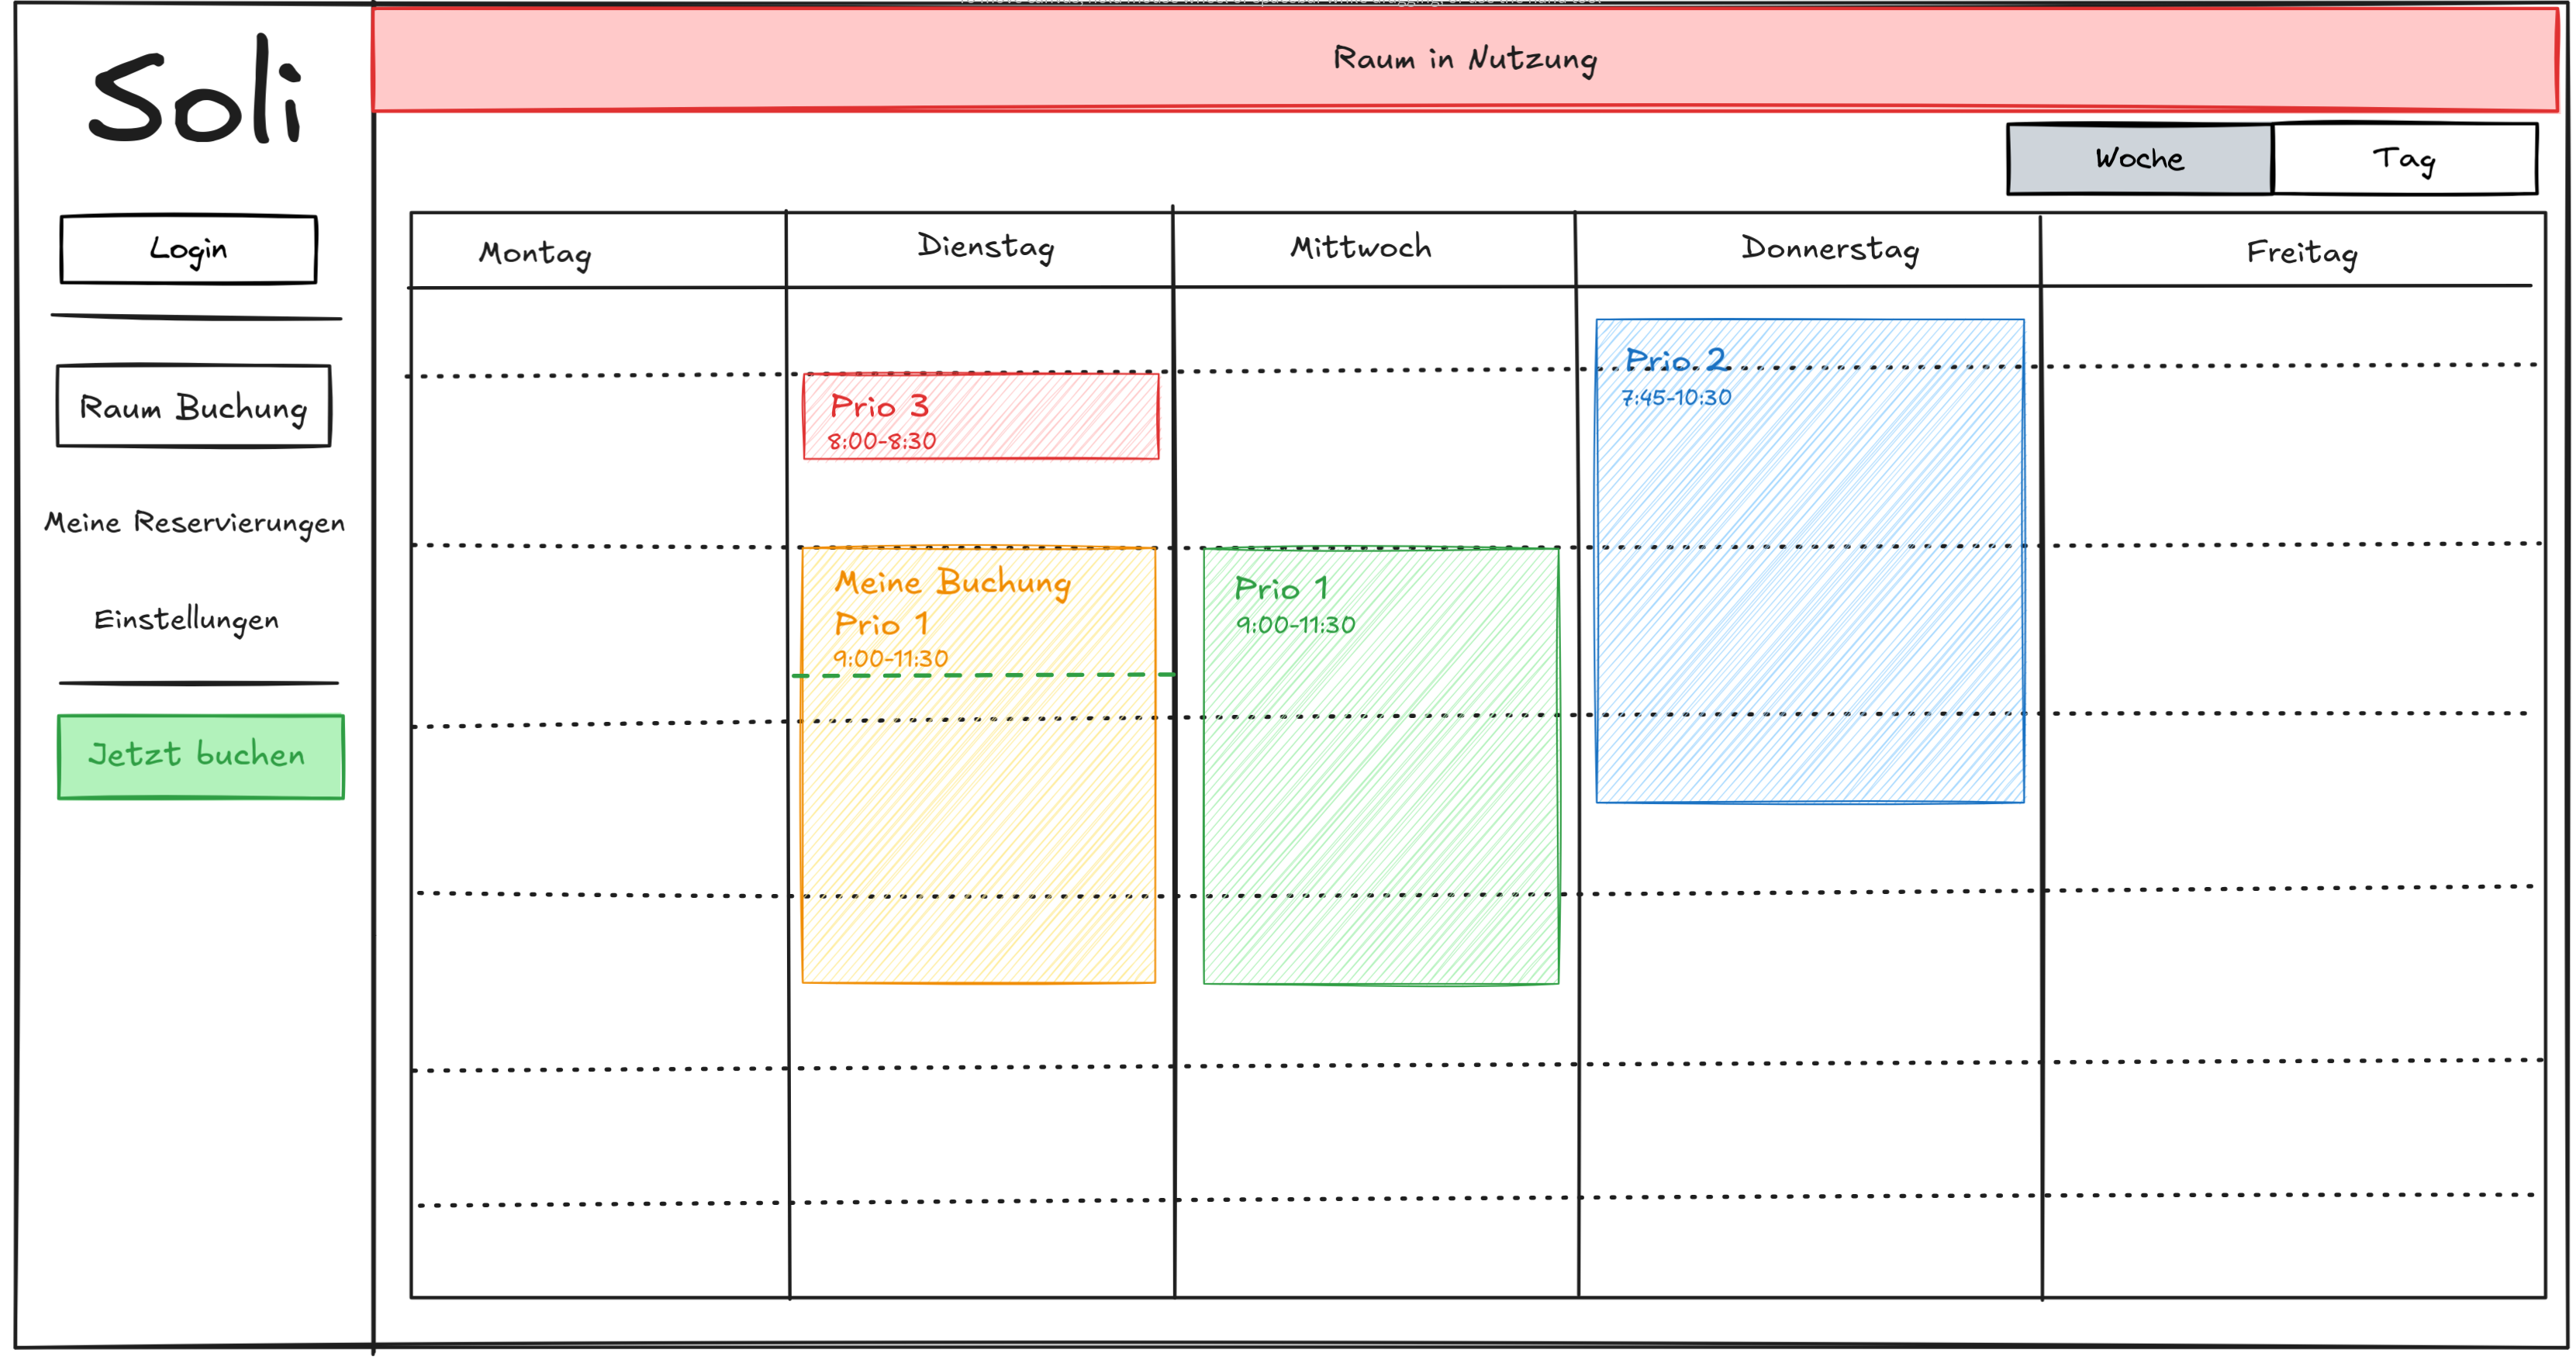
\includegraphics[width=\textwidth]{figures/ui/startseite}
    \caption{Startseite der Anwendung}
    \label{fig:startseite}
\end{figure}
\pagebreak

Sollten Nutzende eine Buchung vornehmen wollen, so klicken diese in den gewünschten Zeitraum
und es wird der Dialog in \ref{fig:buchung} dargestellt.

Der Dialog bietet Nutzenden die Möglichkeit, den genauen Start- und Endzeitpunkt des Termins festzulegen.

Außerdem können Nutzende die Priorität des Termins in Form einer Zahl zwischen 1 und 3 festlegen.
Nutzende können auch angeben, ob sie bereit sind, den Raum mit anderen Nutzenden zu teilen.
Für diesen Zweck werden ihnen drei Optionen bereitgestellt: \textit{Ja}, \textit{Nein} und \textit{Auf Anfrage}.
Siehe dazu auch \ref{fig:buchung}.

Letztlich können Nutzende eine Beschreibung für den Termin hinterlegen, die anderen angemeldeten Nutzenden angezeigt wird.

\begin{figure}[ht]
    \centering
    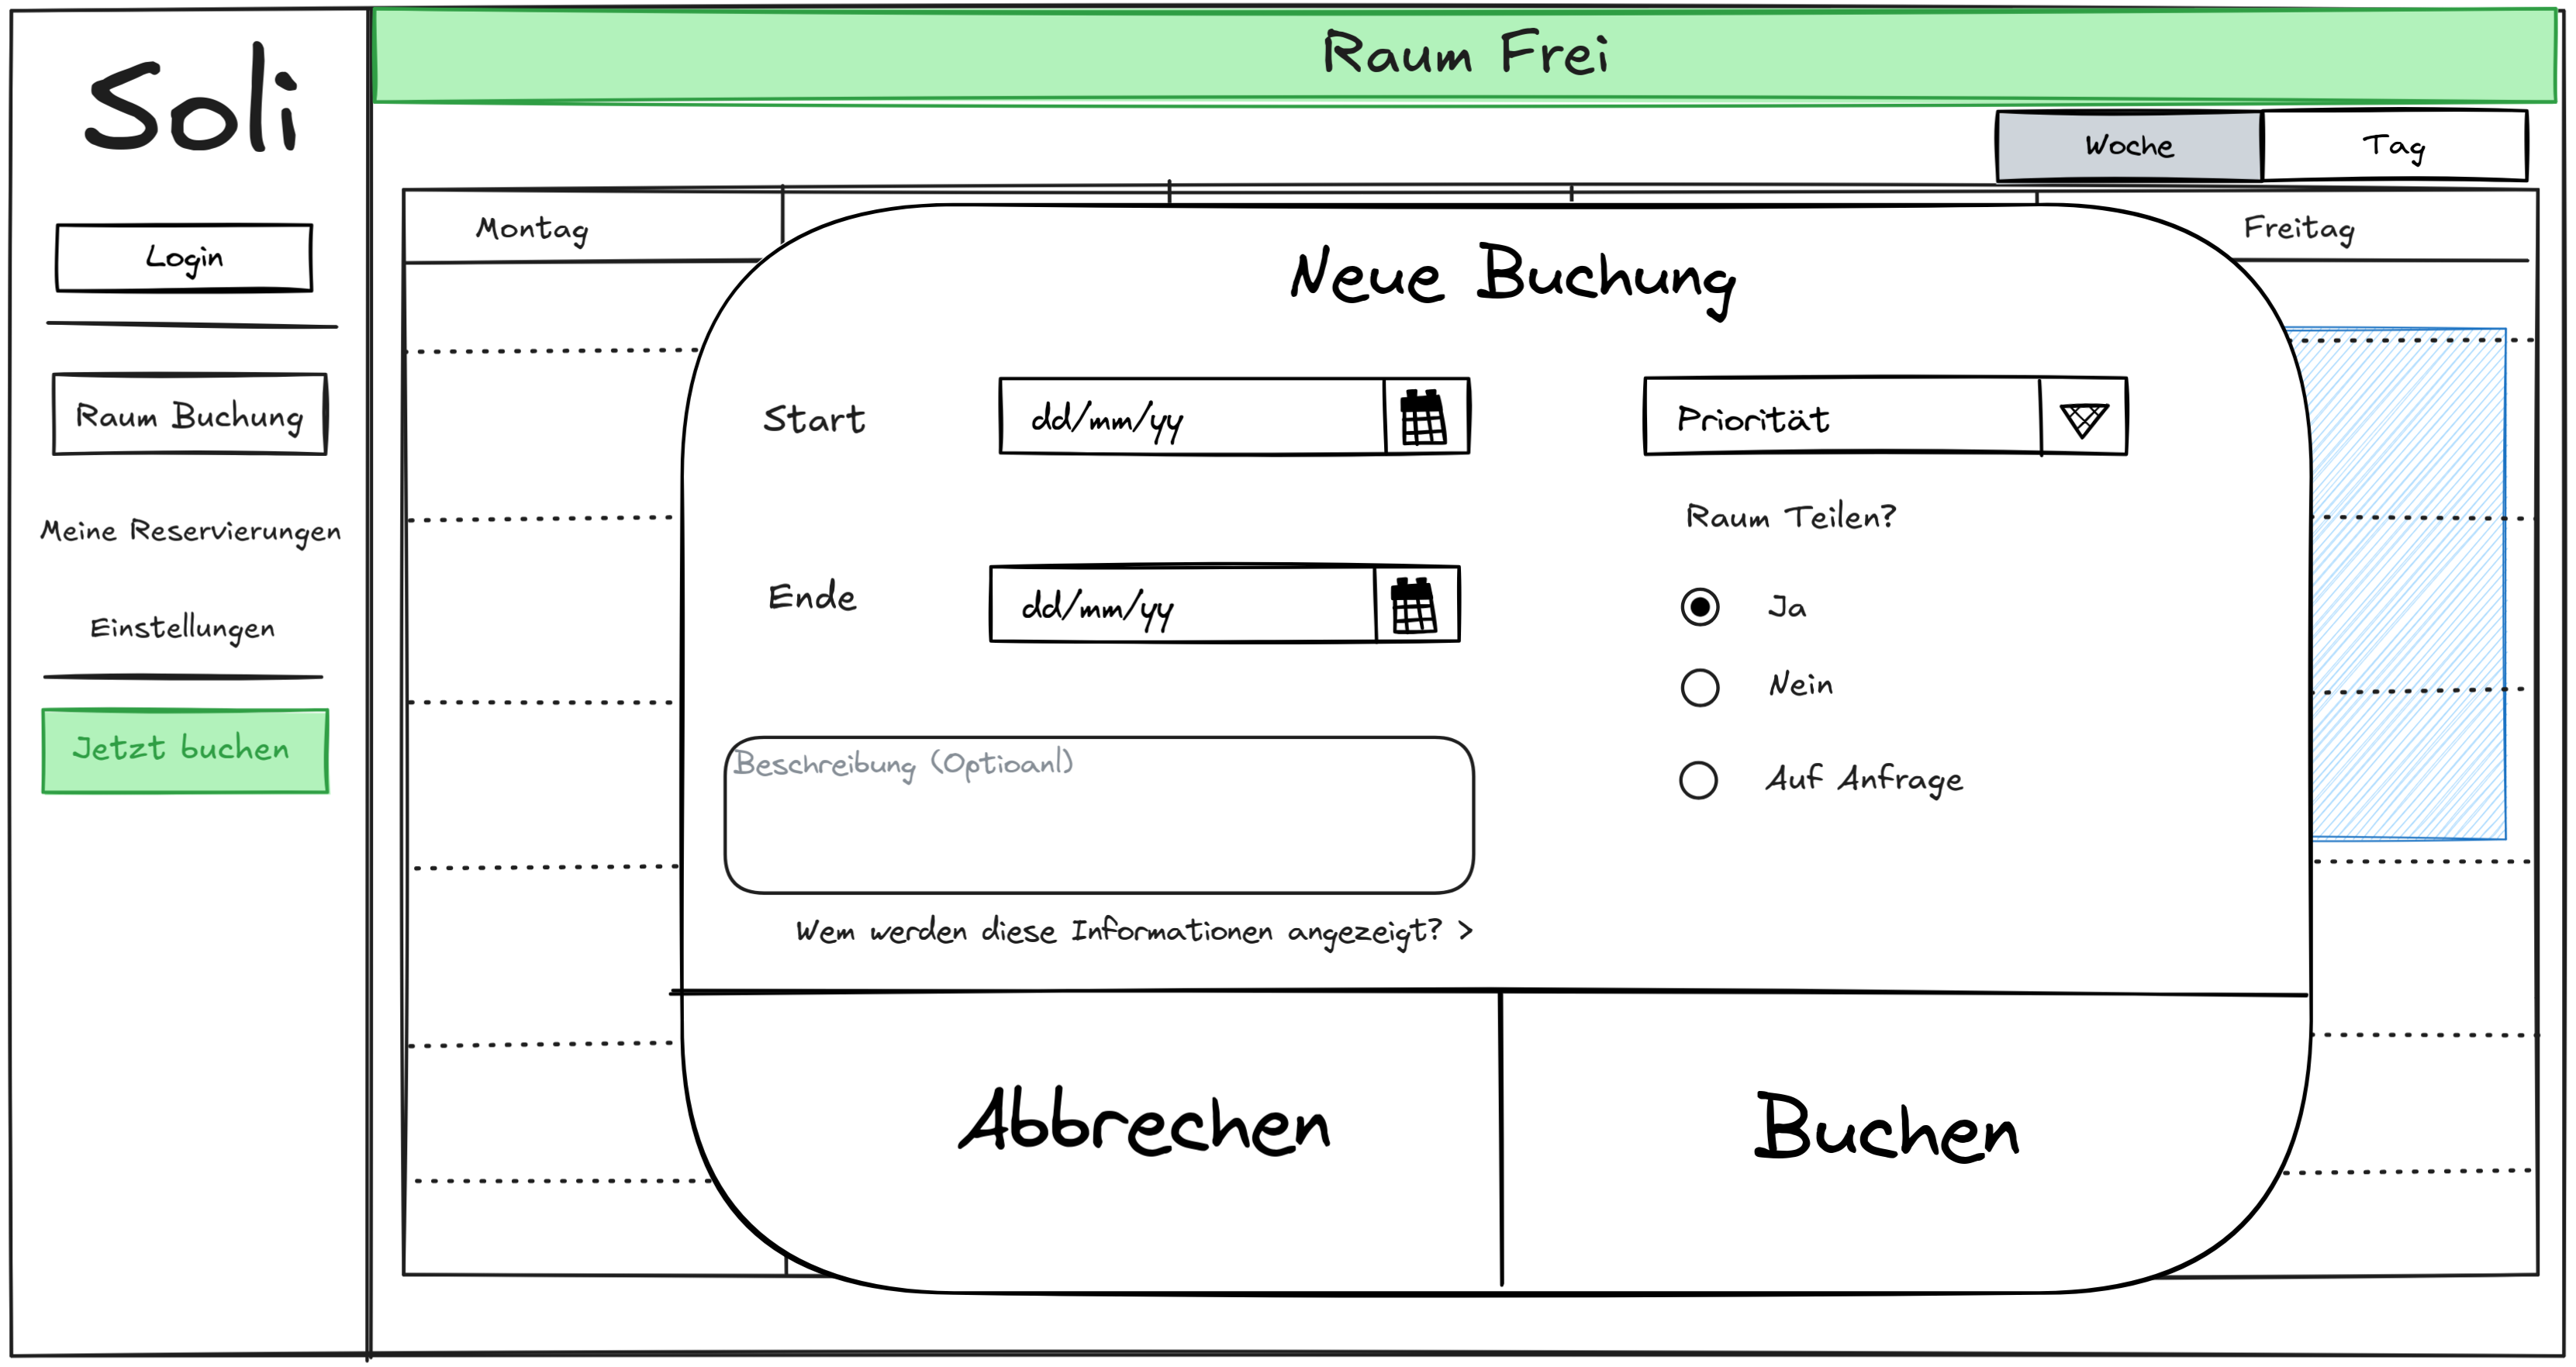
\includegraphics[width=\textwidth]{figures/ui/buchungsdialog}
    \caption{Termin-erstellen}
    \label{fig:buchung}
\end{figure}
\clearpage

Tätigen Nutzende eine Buchung, so werden diese aufgefordert, sich anzumelden.
Der hierzu gehörige Dialog ist in \ref{fig:login} dargestellt.
Alternativ ist dieser Dialog auch über den Anmeldungsbutton, der in Abbildung \ref{fig:startseite} zu sehen ist, erreichbar.

In diesem Dialog wird Nutzenden die Möglichkeit gegeben, sich mit ihrem KIT-Konto, mit einem lokalen Gastkonto oder als Admin anzumelden.

Falls Nutzende die Anmeldung per KIT-Konto wählen, werden sie auf die KIT-Login-Seite weitergeleitet.
Von dort aus können sie sich mit ihren KIT-Zugangsdaten anmelden.

Falls Nutzende die Anmeldung per Gastkonto wählen, werden sie aufgefordert, eine E-Mail-Adresse anzugeben.
Mit der Bestätigung dieser E-Mail-Adresse wird ein temporäres Gastkonto erstellt und die Anmeldung per Cookie gespeichert.

Falls Nutzende die Anmeldung als Admin wählen, werden sie aufgefordert das Passwort des Adminkontos einzugeben.

Nach einer erfolgreichen Anmeldung werden Nutzende auf die nächste Seite weitergeleitet.

\begin{figure}[ht]
    \centering
    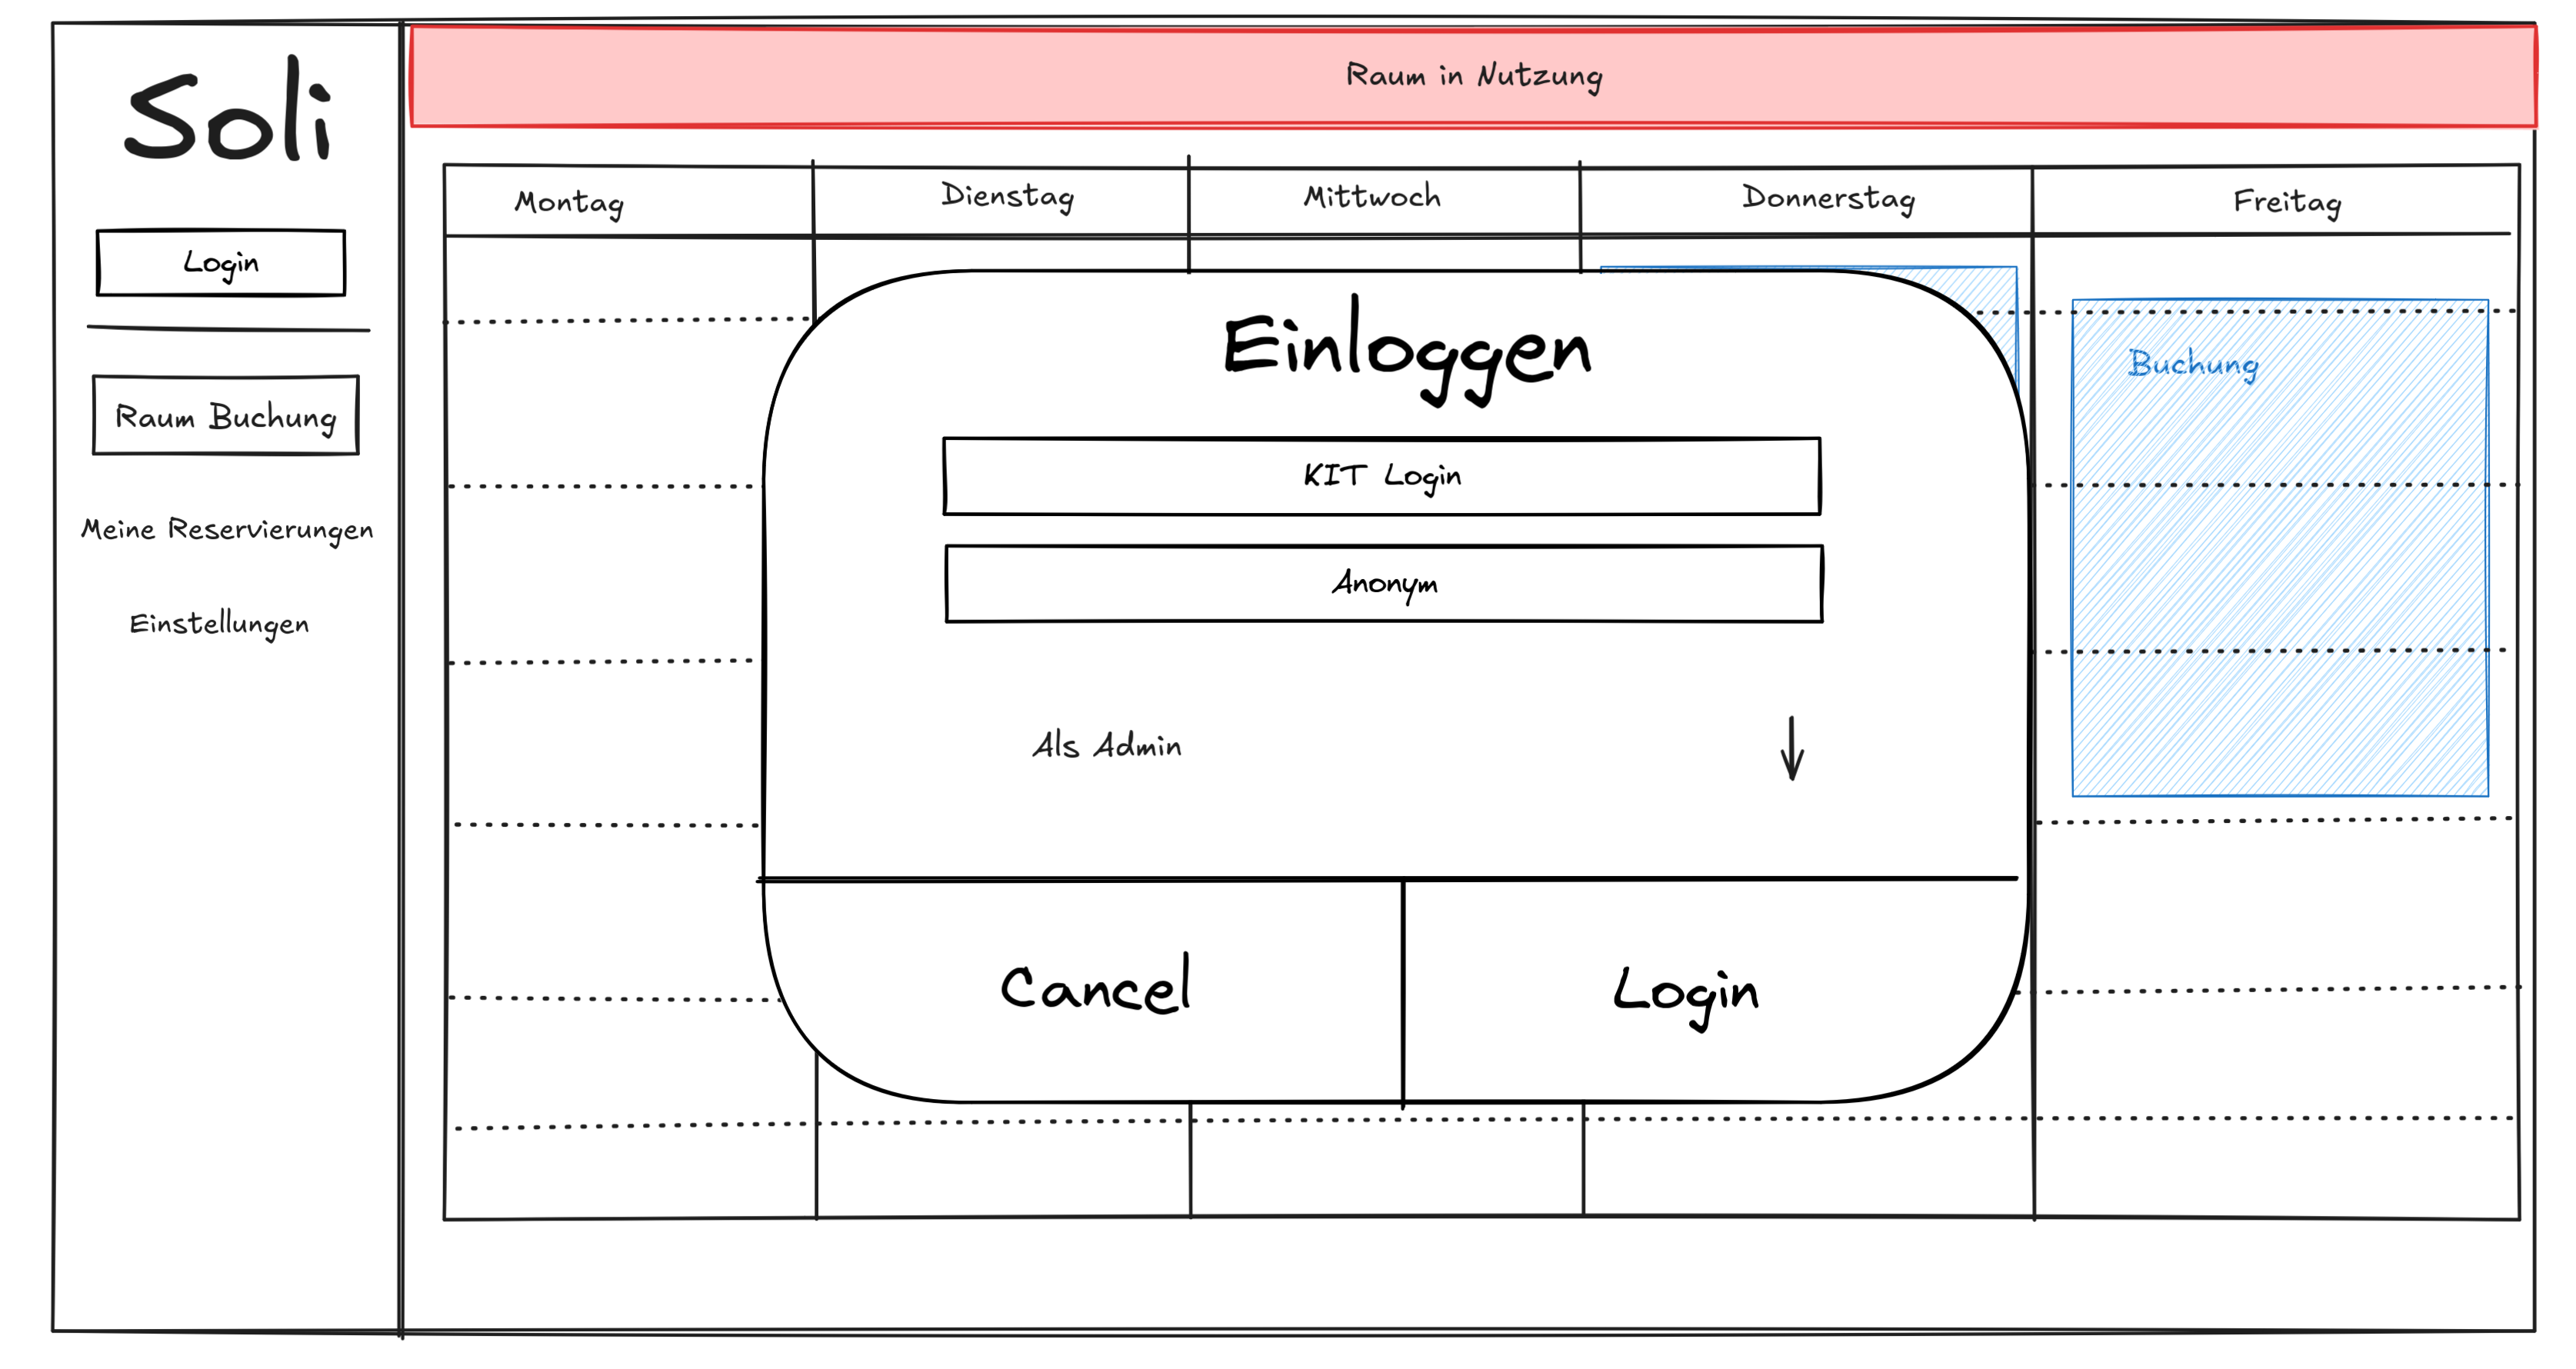
\includegraphics[width=\textwidth]{figures/ui/anmeldungsseite}
    \caption{Anmeldungsseite}
    \label{fig:login}
\end{figure}
\clearpage

Sind Nutzende eingeloggt und belegen den Raum,
so wird ihnen die in Abbildung \ref{fig:checkout} dargestellte Ansicht angezeigt.
Hier können Nutzende den Raum wieder über den Quick-Checkout Button freigeben.


Ziel dieser Ansicht ist es, Nutzenden das frühe Freigeben des Raumes ohne unnötigen Mehraufwand zu ermöglichen.
\begin{figure}[ht]
    \centering
    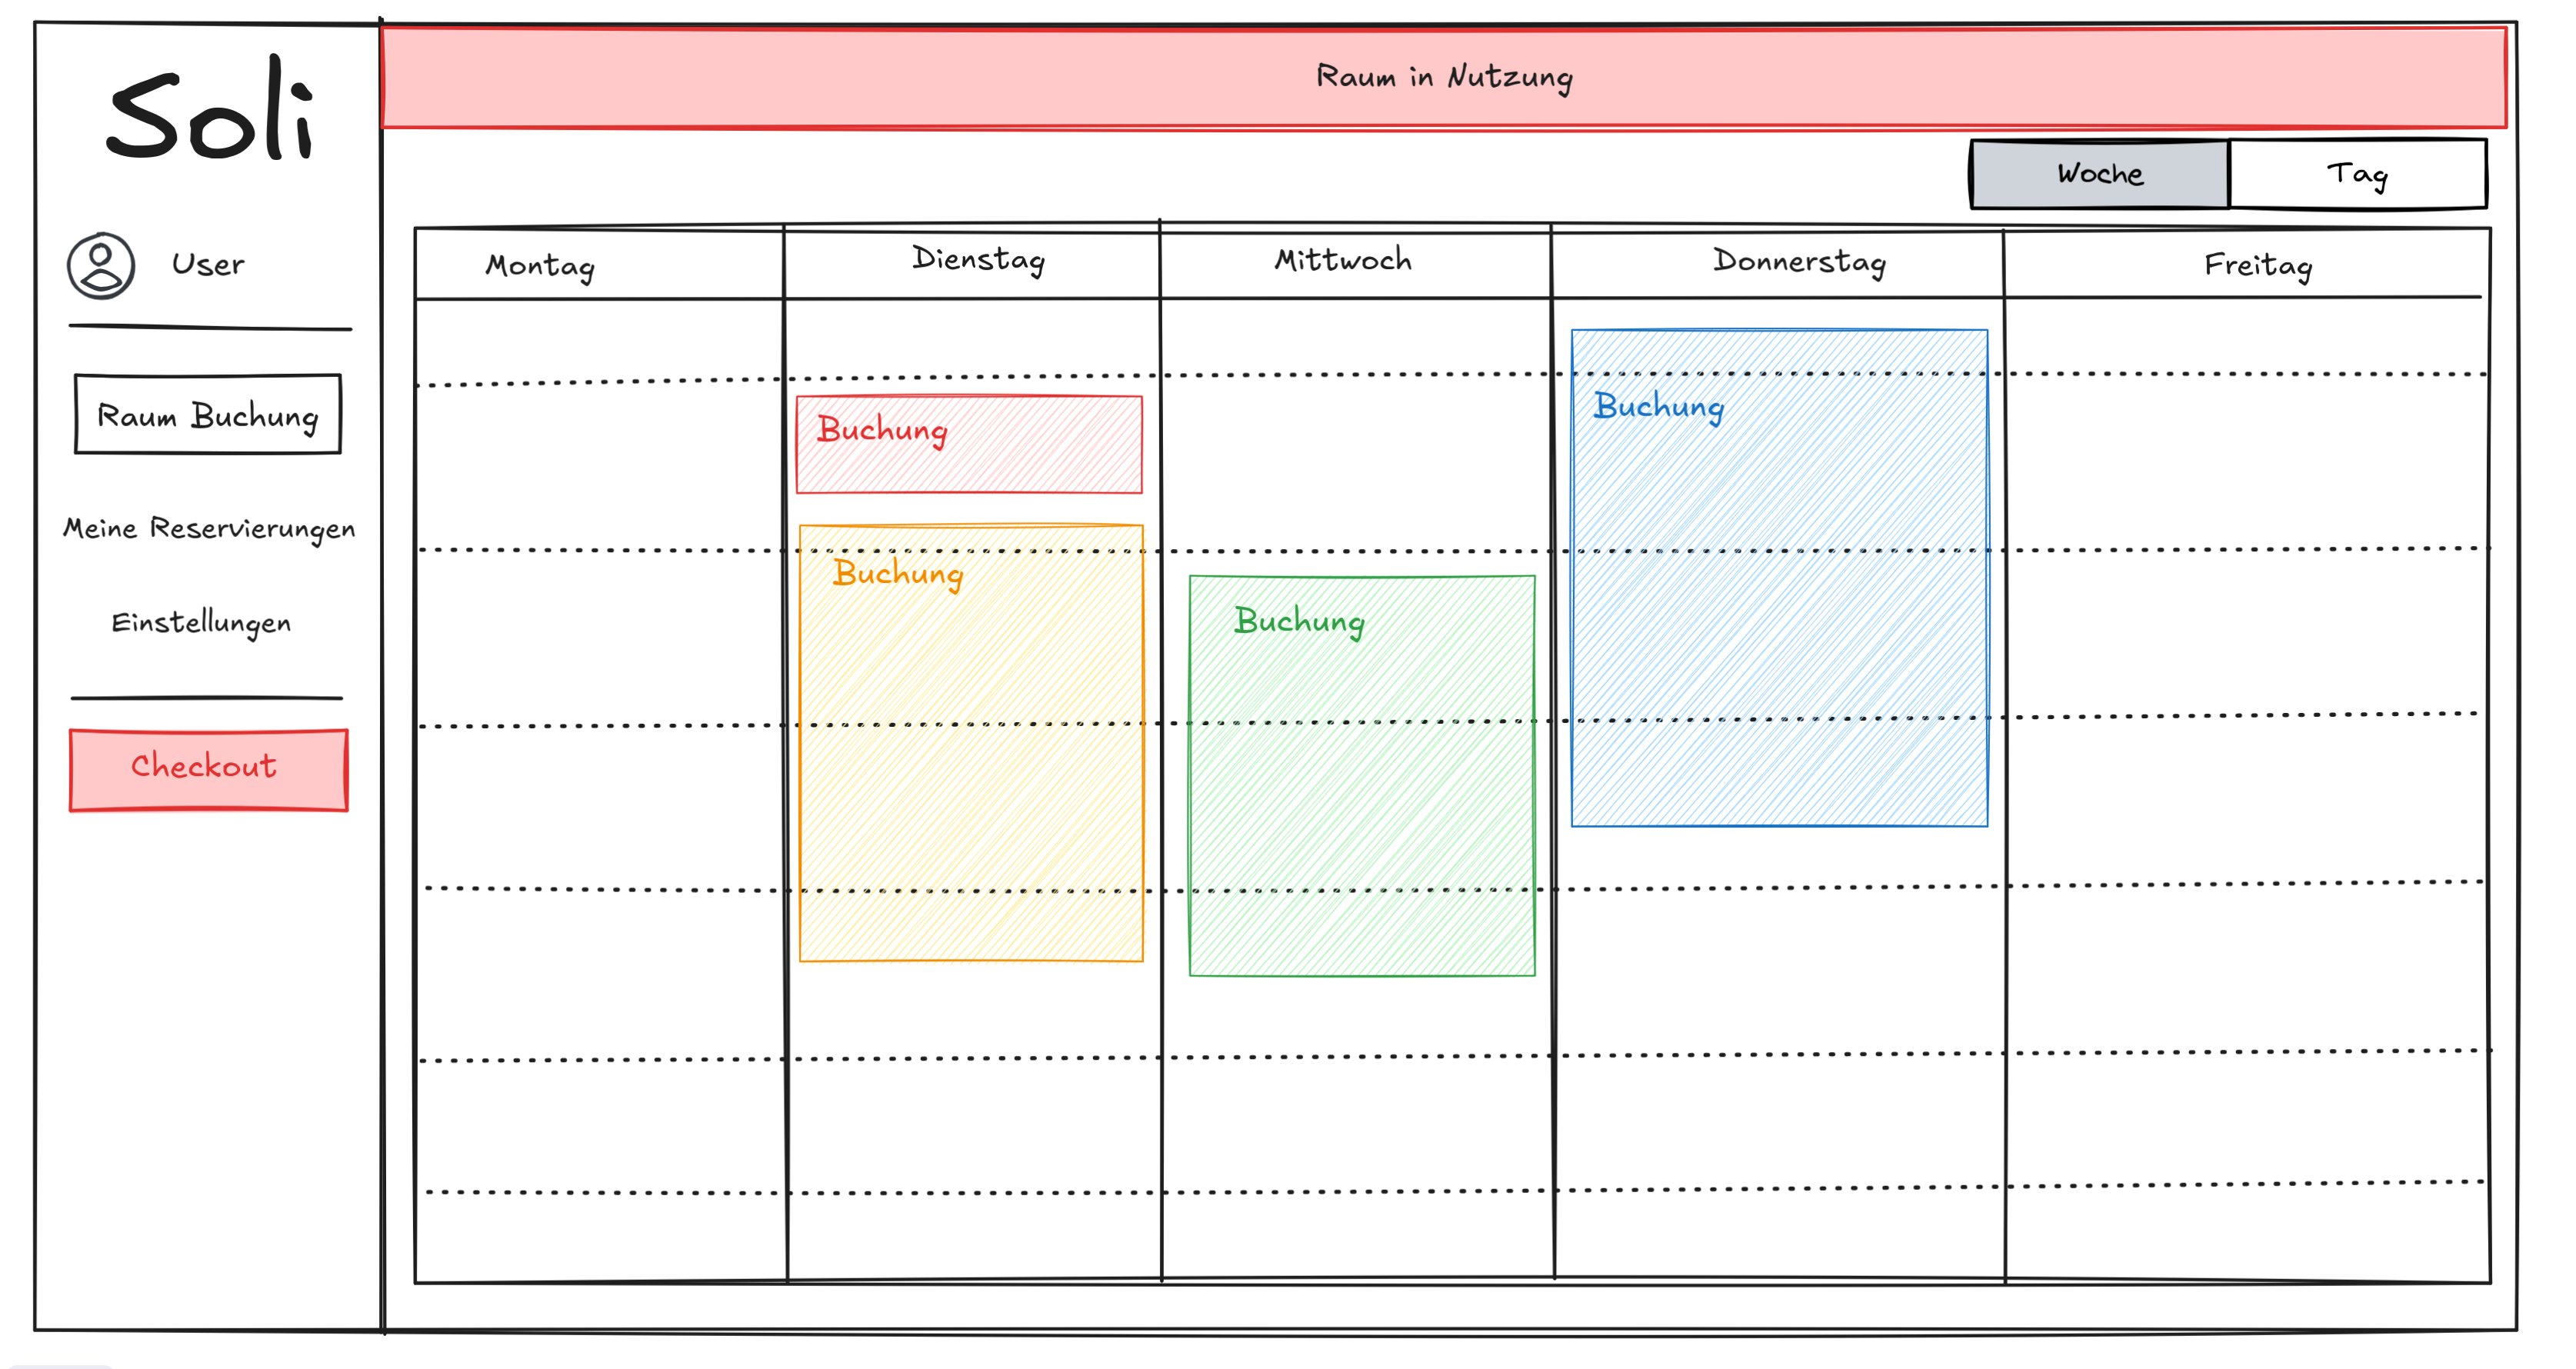
\includegraphics[width=\textwidth]{figures/ui/checkout}
    \caption{Quick Checkout}
    \label{fig:checkout}
\end{figure}
\clearpage

\section{Terminübersicht}
Nutzende, die eine Buchung vorgenommen haben, können diese in der Terminübersicht,
die in Abbildung \ref{fig:overview} dargestellt ist, einsehen und verwalten.

Die Termine in dieser Ansicht werden, anders als in der Ansicht \textit{Kalender}, in Form einer sortierten Liste dargestellt.
Dabei werden die Start- und Endzeitpunkte der Termine, wie auch die Priorität und die Beschreibung angezeigt.

Nutzende haben die Möglichkeit, eine Buchung zu stornieren, indem sie auf den Stornieren-Button klicken.

Außerdem können Nutzende die Ansicht \textit{Termin} (\ref{fig:calendarviewbooking}) zu einem Termin öffnen, indem sie auf den Termin klicken.

\begin{figure}[ht]
    \includegraphics[width=\textwidth]{figures/ui/reservierungsübersicht}
    \caption{Reservierungsübersicht}
    \label{fig:overview}
\end{figure}
\begin{figure}
    \centering
    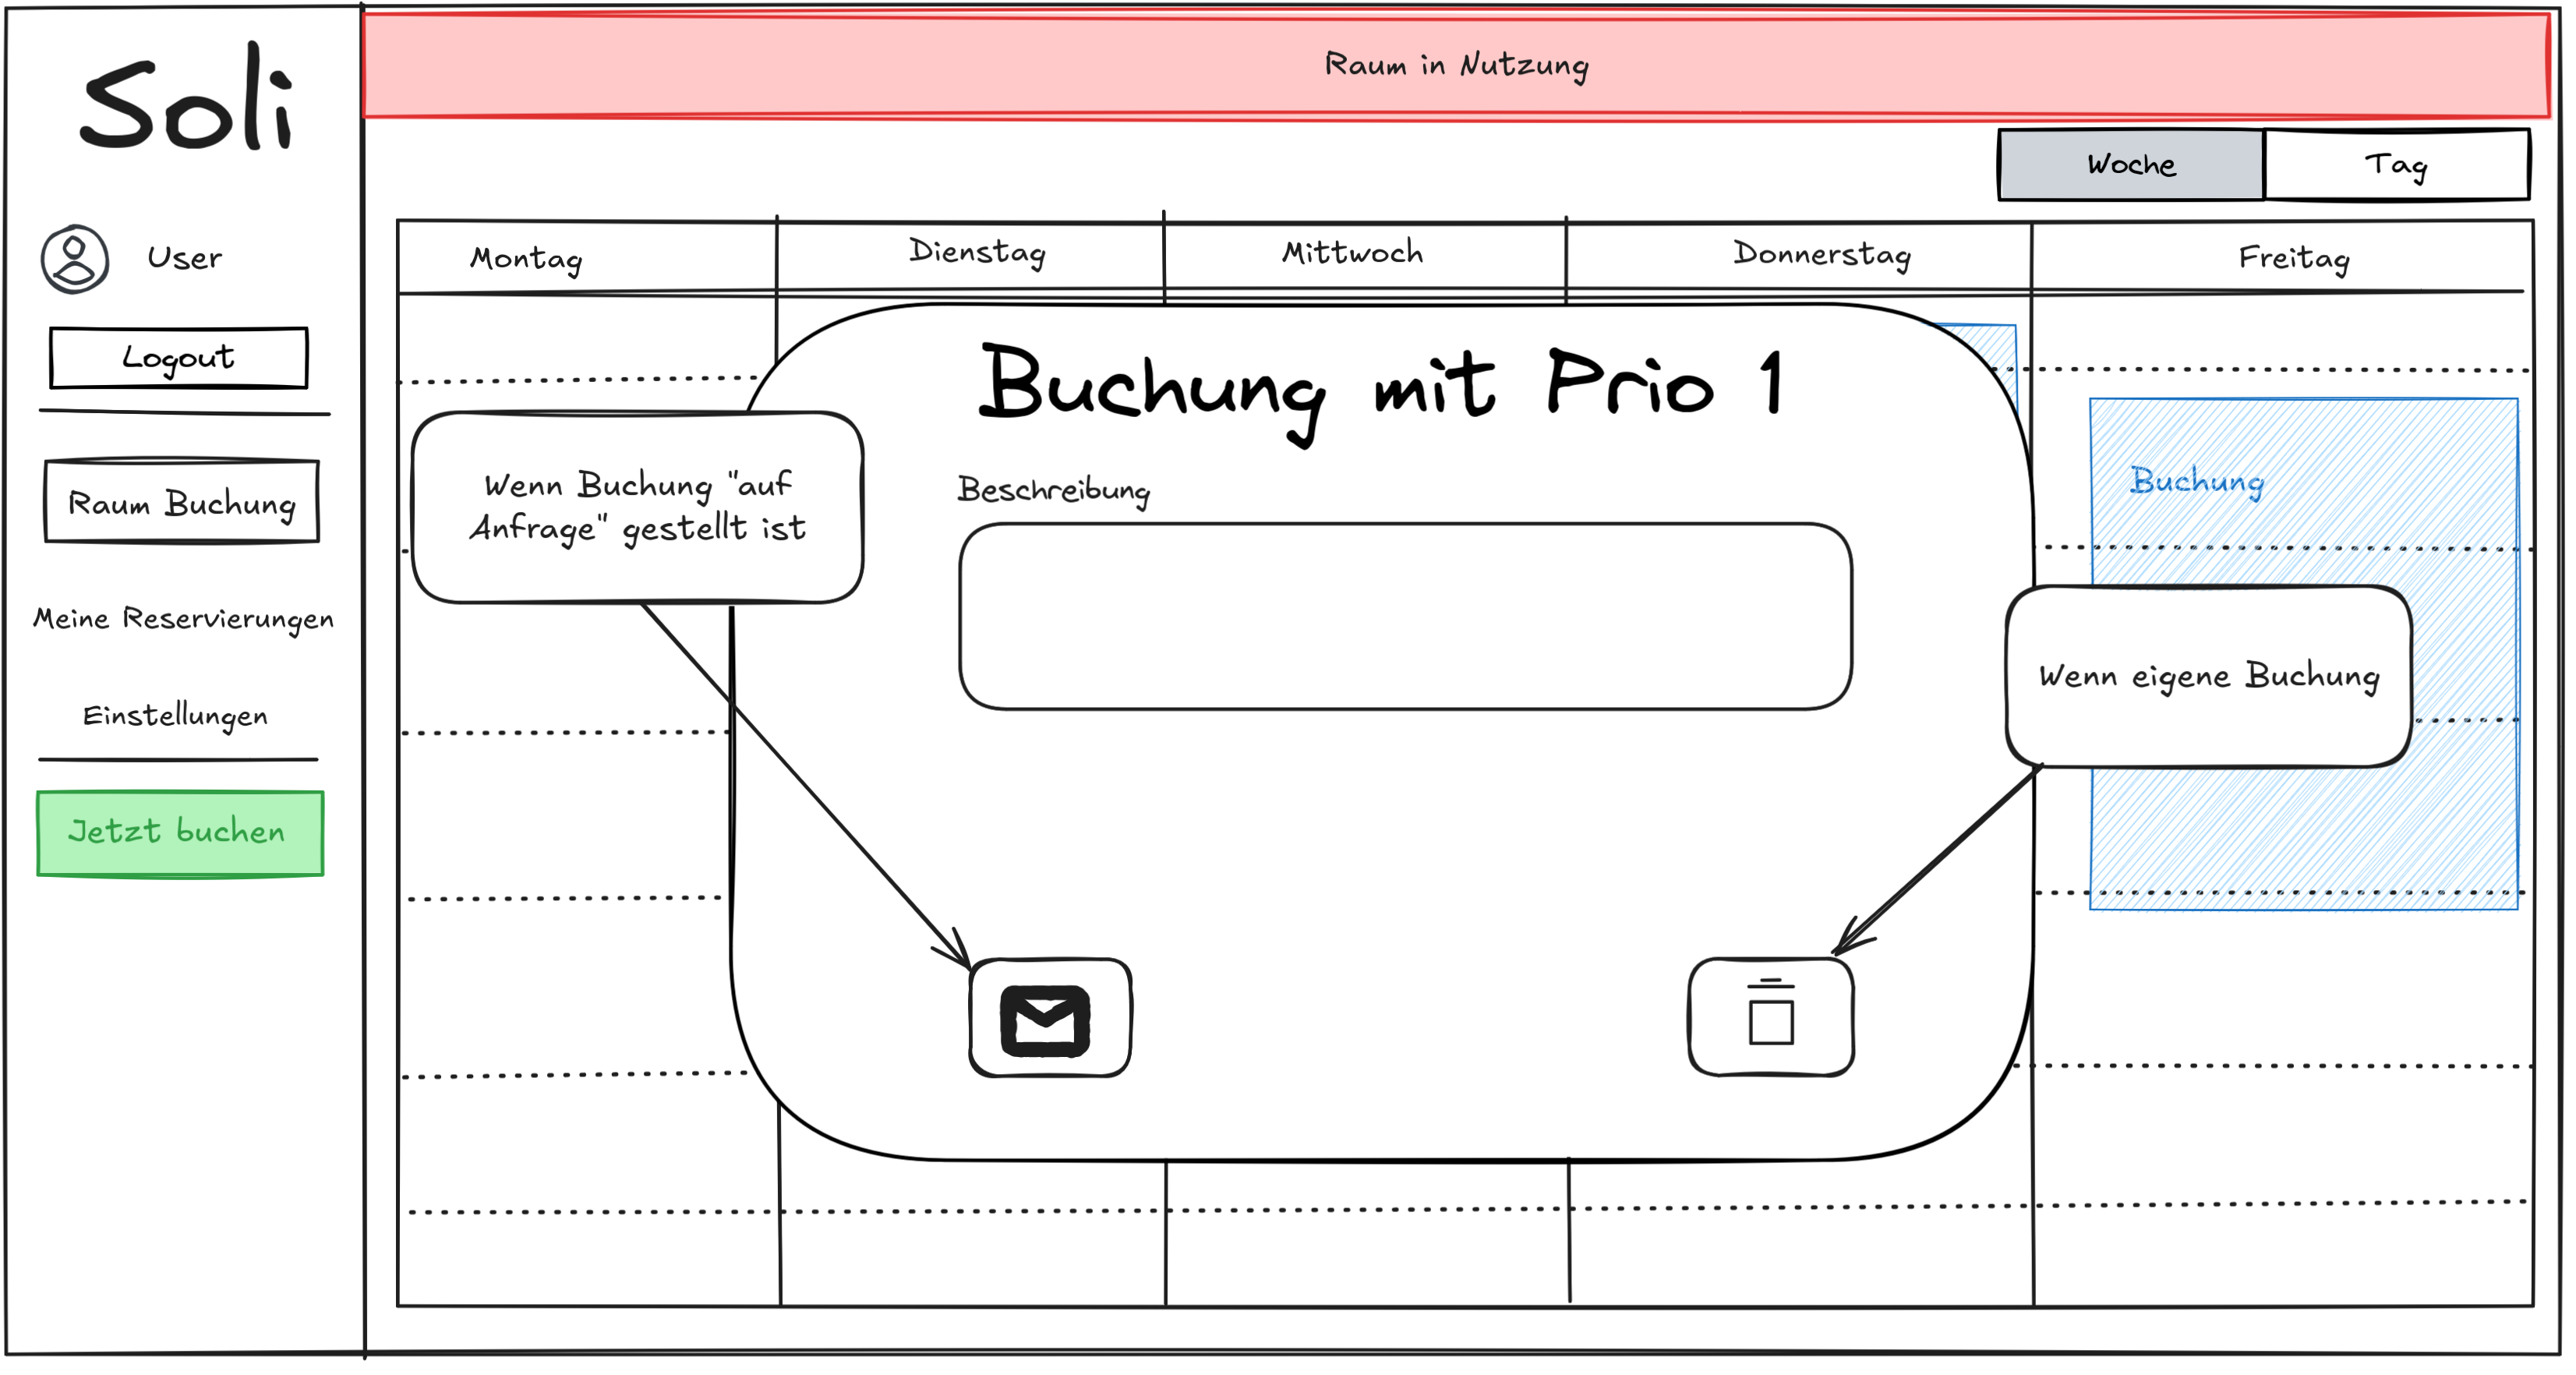
\includegraphics[width=\textwidth]{figures/ui/reservierunginkalendar}
    \caption{Reserverierung im Kalender}
    \label{fig:calendarviewbooking}
\end{figure}
\clearpage

\section{Adminstration}
Ein/e Administrator*in hat die Möglichkeit, über die Benutzeradministrationsoberfläche, die in Abbildung \ref{fig:adminuser} dargestellt ist, Nutzende einzusehen und zu verwalten.

In dieser Ansicht werden alle Nutzenden angezeigt, die sich in der Anwendung registriert haben.
Ein Admin kann die Accounts von Nutzenden deaktivieren und somit ihre Anmeldung verhindern.

Um die Suche nach einem bestimmten Konten zu erleichtern, kann ein Admin nach Kontonamen filtern.

Außerdem kann ein Admin die Anmeldung per Gastkonto deaktivieren.
Zweck dieser Funktion ist es, den Missbrauch von Gastkonten z.B.\ durch Bots in vorübergehenden Zeiten zu verhindern.

\begin{figure}[ht]
    \centering
    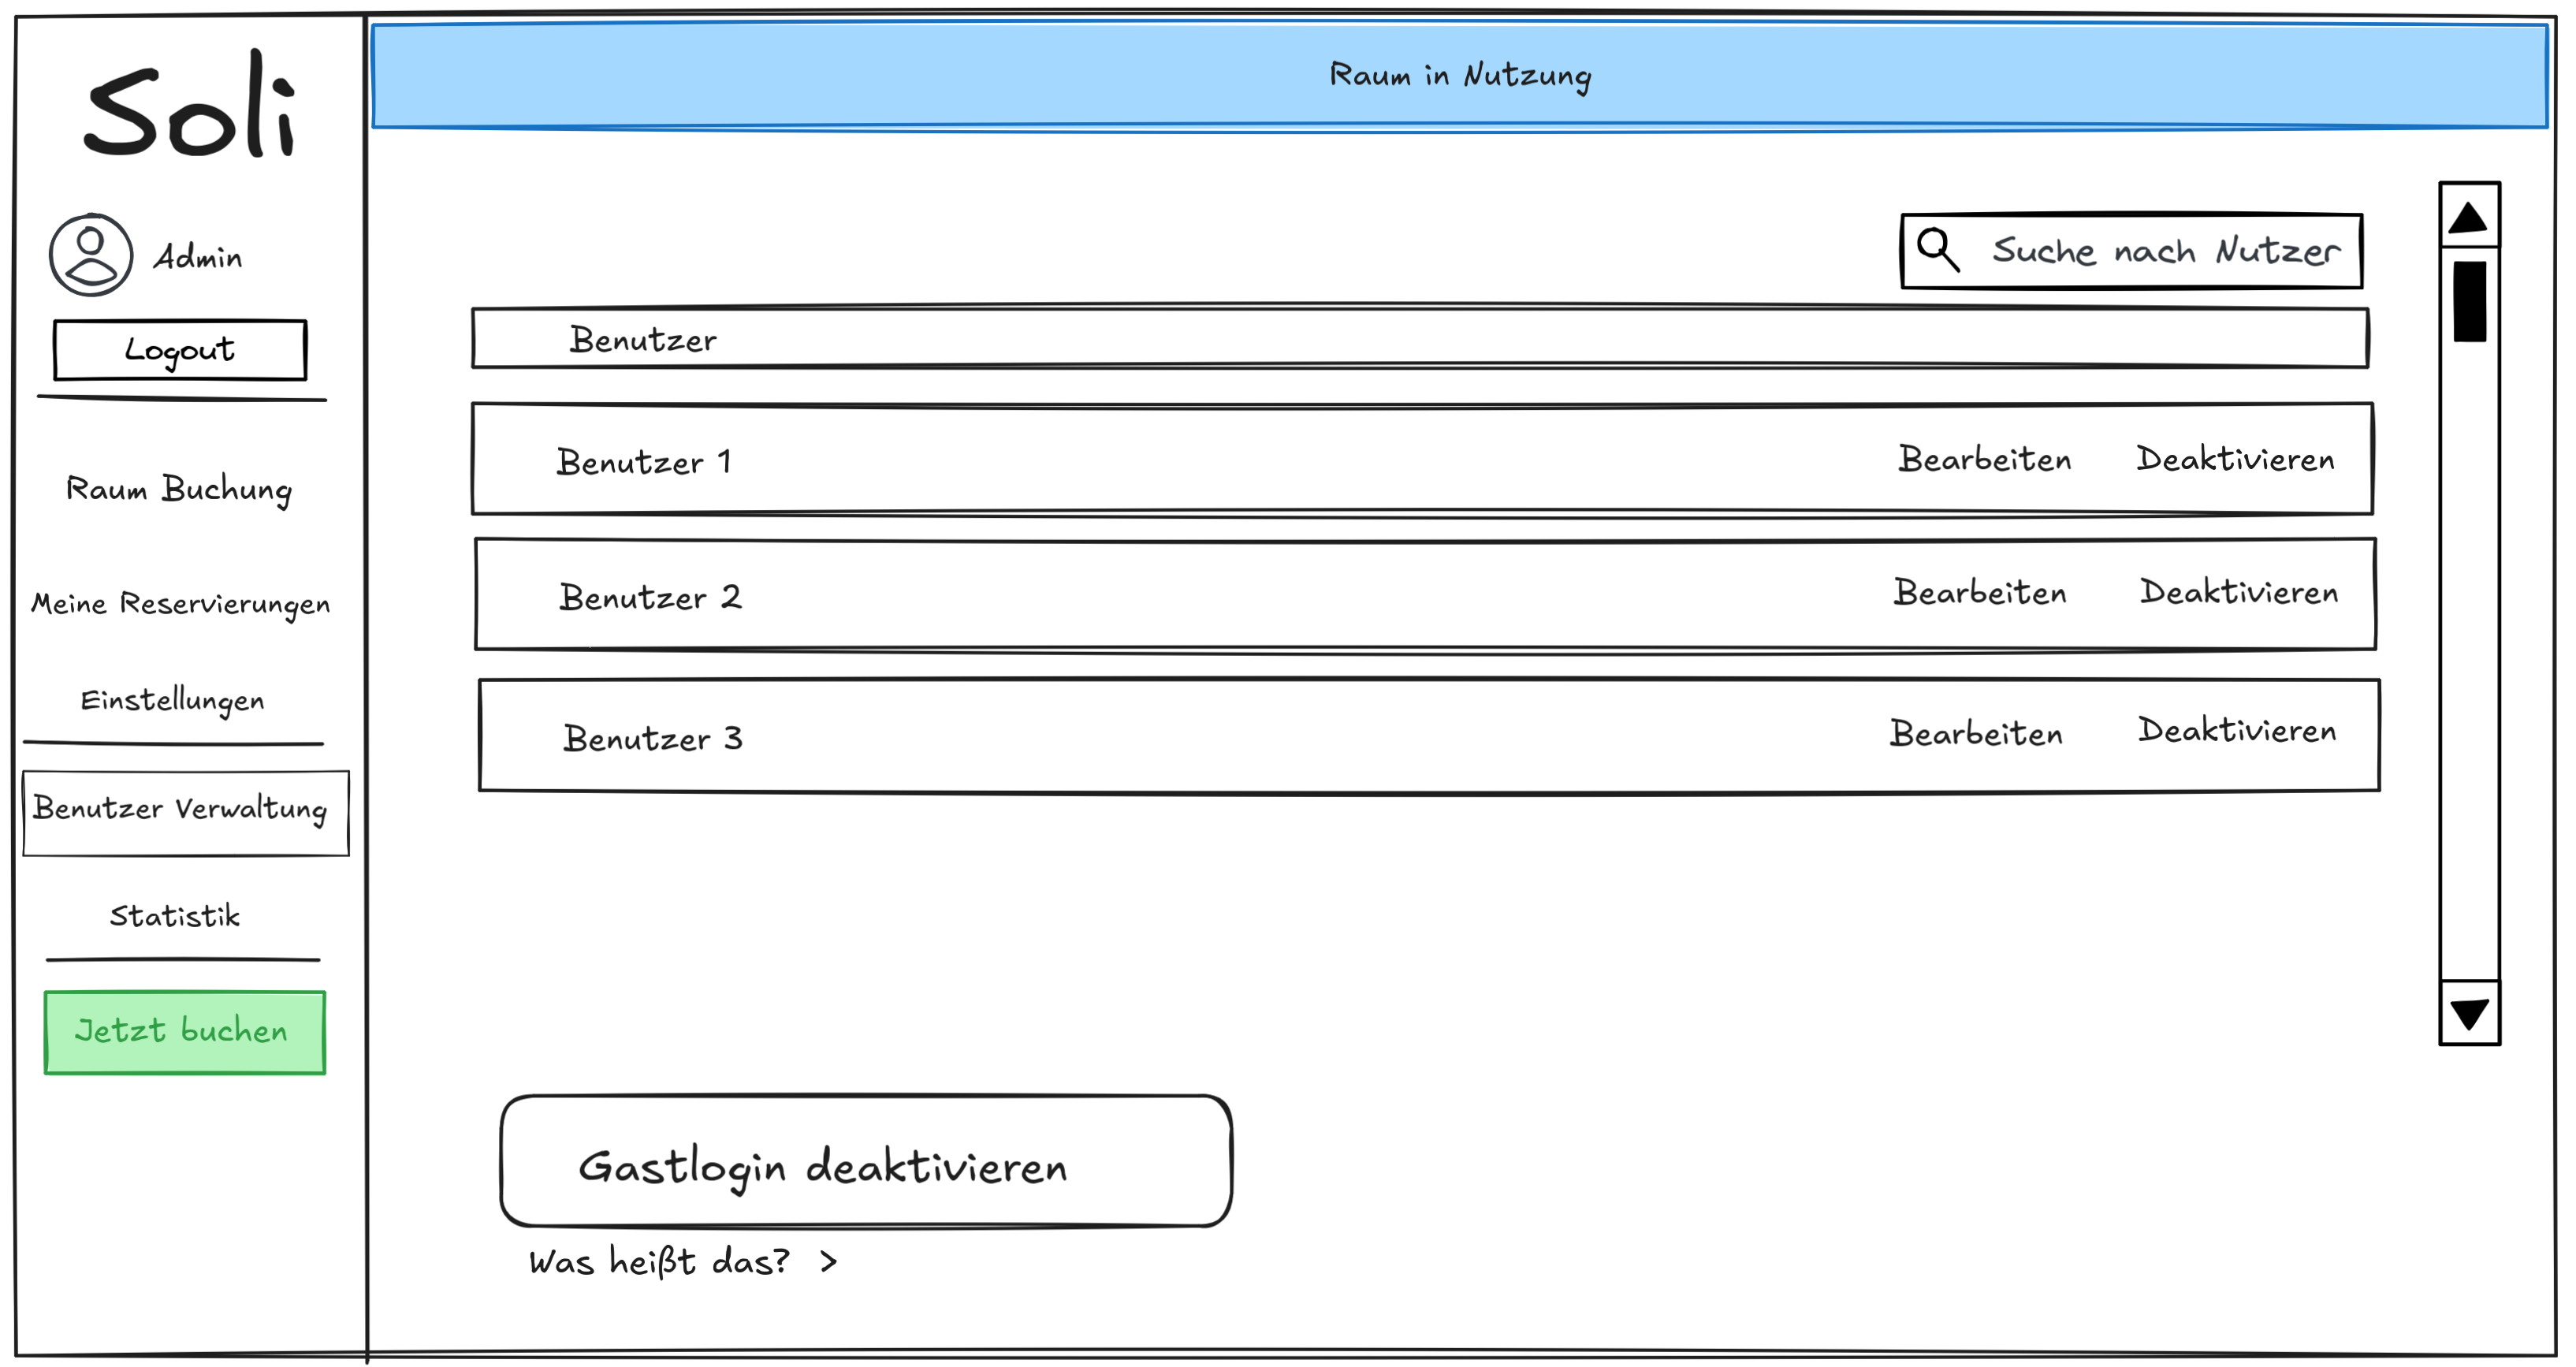
\includegraphics[width=\textwidth]{figures/ui/useradminui}
    \caption{Benutzeradminstrationsoberfläche}
    \label{fig:adminuser}
\end{figure}


%!TEX root = ../Pflichtenheft.tex

% Kapitel 10
% Die Unterkapitel können auch in separaten Dateien stehen,
% die dann mit dem \include-Befehl eingebunden werden.
%-------------------------------------------------------------------------------

\chapter{Technische Produktumgebung}
\label{chap:tech_env}

\section{Entwicklungsumgebung}

\begin{itemize}
    \item \gls{Devcontainer} für reproduzierbare Entwicklungsumgebung
    \item IntelliJ IDEA als \gls{IDE} und LaTex-Editor
    \item pdfLaTeX zur Kompilierung des Dokuments
    \item \gls{Git} zur Versionskontrolle
    \item \gls{Gradle} zur Build-Automatisierung
    \item \gls{GitHub} Actions für \gls{CI} (inkl. Tests und Dokumentation)
    \item \gls{GitHub} Packages zur Speicherung generierter \gls{Docker}-Images
\end{itemize}

\section{Hardware}

\subsection{Backend}

\begin{itemize}
    \item \gls{AMD64}-kompatibler Prozessor (emuliert in einer \gls{VM})
    \item mindestens 1 GB \gls{RAM}
\end{itemize}

\subsection{Frontend}

\begin{itemize}
    \item Beliebiges (mobiles) Gerät mit Internetzugang
\end{itemize}

\section{Software}

\subsection{Backend}

\begin{itemize}
    \item Ubuntu Linux 24.04 LTS als Betriebssystem
    \item \gls{Docker} zur \gls{Container}isierung der Anwendung
    \item \gls{PostgreSQL} als Datenbank (in einem eigenen \gls{Container})
    \item Applikations-\gls{Container} (gebaut in \gls{CI})
    \item Spring Boot mit Java 21 als Backend-Framework
    \item JTE zur Generierung von \gls{HTML}-Seiten
    \item Caddy als HTTPS-Reverse-Proxy
\end{itemize}

\subsection{Frontend}

\begin{itemize}
    \item Pure \gls{HTML} mit \gls{JavaScript} zur Interaktivität um maximale Kompatibilität zu gewährleisten
    \item Vorgefertigtes \gls{CSS}-Framework für konsistentes Design
    \item FullCalendar für den Kalender
    \item Moderner \gls{Browser} (Chrome, Firefox, Safari, Edge) zur vollen Funktionalität
\end{itemize}

\section{Schnittstellen}

\begin{itemize}
    \item \gls{SSR} generiert (hauptsächlich) statische \gls{HTML}-Seiten
    \item \gls{HTML}-Forms zur Interaktion mit dem Backend
    \item Minimale \gls{REST}-\gls{API} zum Prüfen auf Verfügbarkeit
\end{itemize}
\chapter{Testfälle und Testeszzenarien}
\label{chap:test}
In diesem Kapitel definieren wir die Testfälle und Testfallszenarien.

\section{Testfälle}

\begin{table}[htbp]
  \centering
  \begin{tabularx}{\textwidth}{ l|X|l }
      \textbf{Nr.} & \textbf{Beschreibung} & \textbf{Funktion} \\ \hline\hline
      ⟨T10⟩ & Landeseite besuchen &\ref{F10}\\
      ⟨T20⟩ & Login &\ref{F20} \\
      ⟨T30⟩ & Abmelden &\ref{F30} \\
      ⟨T40⟩ & Reservieren &\ref{F40} \\
      ⟨T50⟩ & Löschen von Terminen durch Administratoren &\ref{F50} \\
      ⟨T60⟩ & Deaktivieren eines Kontos &\ref{F60} \\
      ⟨T70⟩ & Benachrichtigung bei freiem Raum &\ref{F70} \\
      ⟨T80⟩ & Anzeige des Raumstatus &\ref{F80} \\
      ⟨T90⟩ & Stornierung einer Reservierung &\ref{F90} \\
      ⟨T100⟩ & Login mit Adminkonto &\ref{F100} \\
      ⟨T110⟩ & Deaktivierung von Gastkonten &\ref{F110} \\
      ⟨T120⟩ & Öffnungszeiten einstellen &\ref{F120} \\
      ⟨T130⟩ & Terminkonfliktauflösung &\ref{F130} \\
  \end{tabularx}
  \caption{Überblick der Testfälle.}
  \label{tab:test_table}
\end{table}

\pagebreak

\section{Testfallszenarien}\label{sec:testfallszenarien}
\begin{scenario}{10}{Besuch der Landeseite und Anmeldung/Abmeldung}
  \item[Ziel:] Sicherstellen, dass Nutzende die Landeseite aufrufen und sich erfolgreich anmelden bzw.\ abmelden können.
  \begin{enumerate}
    \item Der Nutzende besucht die Landeseite ⟨T10⟩.
    \item Der Nutzende loggt sich ein ⟨T20⟩.
    \item Der Nutzende meldet sich ab ⟨T30⟩.
  \end{enumerate}
\end{scenario}

\begin{scenario}{20}{Reservierung eines Raums und Stornierung}
  \item[Ziel:] Überprüfen, ob Nutzende erfolgreich Termine reservieren können.
  \begin{enumerate}
    \item Der Nutzende besucht die Landeseite ⟨T10⟩.
    \item Der Nutzende meldet sich an ⟨T20⟩.
    \item Der Nutzende wählt einen verfügbaren Raum aus und reserviert diesen ⟨T40⟩.
    \item Buchen ausserhalb der Öffnungszeiten sollte hierbei fehlschlagen.
    \item Überprüfen, ob der Raumstatus korrekt angezeigt wird und sich ggf.\ geändert hat ⟨T80⟩.
    \item Der Nutzende storniert die Reservierung ⟨T90⟩.
    \item Andere Nutzende, welchen sich diesen Termin vorgemerkt hatten, werden benachrichtigt, dass der Raum nun Frei ist ⟨T70⟩.
  \end{enumerate}
\end{scenario}

\begin{scenario}{30}{Terminverwaltung durch das Adminkonto}
  \item[Ziel:] Testen der administrativen Funktionalitäten zum Löschen von Terminen.
  \begin{enumerate}
    \item Ein Admin besucht die Landeseite ⟨T10⟩.
    \item Der Admin meldet sich an ⟨T100⟩.
    \item Der Admin löscht bestehende Termine ⟨T50⟩.
    \item Der Admin meldet sich ab ⟨T30⟩.
  \end{enumerate}
\end{scenario}

\pagebreak

\begin{scenario}{40}{Kontoverwaltung durch das Adminkonto}
  \item[Ziel:] Testen der administrativen Funktionalitäten zum Deaktivieren von Gastkonten und einstellen der Öffnungszeiten.
  \begin{enumerate}
    \item Ein Admin besucht die Landeseite ⟨T10⟩.
    \item Der Admin meldet sich an ⟨T100⟩.
    \item Der Admin deaktiviert die Anmeldung von Gastkonten ⟨T110⟩.
    \item Der Admin ändert die Öffnungszeiten für einen bestimmten Wochentag ⟨T120⟩.
    \item Der Admin öffnet die Ansicht \textit{Kontoliste} und deaktiviert ein Konto ⟨T60⟩.
    \item Der Admin meldet sich ab ⟨T30⟩.
    \item Das Anmelden mit einem Gastkonto sollte jetzt fehlschlagen ⟨T20⟩.
    \item Das Anmelden mit dem deaktiviertem Konto sollte ebenfalls fehlschlagen ⟨T20⟩.
    \item Die Ansicht \textit{Kalender} sollte die neuen Öffnungszeiten darstellen.
  \end{enumerate}
\end{scenario}

\begin{scenario}{50}{Terminkonflikt auflösung}
  \item[Ziel:] Überprüfen, ob ein Terminkonflikt richtig aufgelöst wird.
  \begin{enumerate}
    \item Konto 1 meldet sich an ⟨T20⟩.
    \item Konto 1 erstellt einen Termin, und gibt die zu testende Priorität, Raumteilungsoption und Zeitperiode ein ⟨T20⟩.
    \item Konto 1 meldet sich ab und Konto 2 meldet sich an.
    \item Konto 2 erstellt einen Termin, welcher den anderen überlappt.
    \item Es wird überprüft, ob die erwartete Konfliktauflösung stattgefunden hat und ggf.\ die dafür benötigten E-Mails versendet wurden ⟨T130⟩.
  \end{enumerate}
\end{scenario}

\printglossaries

%------Ende des Dokumentes------------------------------------------------------
\end{document}
